\documentclass[12pt]{scrartcl}
\usepackage[sexy]{evan}
\usepackage{quiver}

\newcommand{\Ann}{\mathrm{Ann}}
\newcommand{\Ass}{\mathrm{Ass}}
\newcommand{\Lt}{\mathrm{Lt}}
\renewcommand\AA{\mathbb{A}}
\renewcommand\qedsymbol{$\mathfrak{Q.E.D.}$}
\usepackage{relsize}
\begin{document}
\title{Note on Commutative Algebra}
\author{Jiawen Huang}
\maketitle
\newpage
\tableofcontents
\newpage
\section*{Acknowledgement}
\begin{enumerate}
\item This note is basically a copy of Eisenbud's Commutative Algebra with a View Toward Algebraic Geometry, with some additional explanations and examples from Eisenbud's lectures and my own understanding.
\item This latex style is made by Evan Chen. 
\item In this note, all rings $R$ are commutative with unity unless otherwise specified.
\item When we use the language of category theory, we are in $R$-modules categories unless otherwise specified.
\item We assume the Axiom of Choice/Zorn's Lemma. 
\end{enumerate}

\newpage 

\section{January 17, 2026: A theorem in Invariant Theory}
\begin{corollary}[Summand of polynomial rings over fields is finitely generated]
    Let $k$ be a field, and let $R$ be a $k$-subalgebra of $S=k[x_1, \ldots, x_n]$. $R$ is a direct summand of $S$ in the sense that there is a surjective $R$-algebra homomorphism $\phi: S \to R$ such that $\phi|_R = \mathrm{id}_R$ and $\phi$ preserves degrees. Then $R$ is finitely generated as a $k$-algebra.
\end{corollary}
\begin{proof}
    Intuition: $R$ itself is a graded $k$-algebra, with grading inherited from $S$. As a graded algebra, $R$ can be decomposed into its homogeneous components. $R_0$ is easy to get, just include $1$ in the generators. Therefore, to generate $R$, we really need to generate the positive degree part. That motivates us to look at the ideal $R_+$. 
    \\

    But $R_+$ may not be finitely generated as an ideal. However, we know that $S$ is a Noetherian ring, so we can look at the ideal $R_+S$. It must be finitely generated, say by $f_1, \ldots, f_m \in R_+$.
    \\

    Now, we claim that $R=k[1,f_1, \ldots, f_m]$. Certainly, the right hand side is contained in the left hand side. For the other direction, it suffices to show that any homogeneous element of $R$ can be generated by $f_1, \ldots, f_m$ with coefficients in $k$. We prove this by induction on degree $d$. $d=0$ is trivial. Now suppose we have shown this for degree less than $d$. Take any homogeneous element $r \in R$ of degree $d$. Since $r \in R_+S$, we can write $r=\sum g_if_i$ for some homogeneous element $g_i \in S$. Apply $\phi$ to both sides, we get
    \[r=\phi(r)=\sum \phi(g_i)\phi(f_i)=\sum \phi(g_i)f_i.\]
    Note that $\deg(\phi(g_i))=\deg(g_i) < d$, so by the inductive hypothesis, each $\phi(g_i)$ can be generated by $f_1, \ldots, f_m$ over $k$. Therefore, $r$ can also be generated by $f_1, \ldots, f_m$ over $k$. This finishes the proof.
\end{proof}
\begin{remark}
    This shows that the invariant ring of a linearly reductive group acting on a polynomial ring over a field is finitely generated. If the group $G$ is finite, the surjective homomorphism $\phi$ can be taken as $\phi(f)=\sum_{g \in G} gf$. (Weyl's averaging trick)
\end{remark}
\begin{remark}
    Graded rings are great because it allows us to use induction on degree. So we only need to worry about homogeneous elements. 
\end{remark}
\newpage
\section{January 20, 2026: Basis, syzygy, and Hilbert's function theorems}
First day of Commutative Algebra course!

We discuss the history of Commutative Algebra and three of the four big theorems. 

\begin{theorem}[Hilbert's Basis Theorem]
    If $R$ is a Noetherian ring, then the polynomial ring $R[x]$ is also Noetherian.
\end{theorem}
\begin{proof}
    Let $I$ be an ideal of $R[x]$. Our goal is to show that $I$ is finitely generated. We first pick the smallest degree nonzero polynomial $f_1$ in $I$. Next, we take $f_2$ to be the smallest degree polynomial in $I$ which is not in the ideal generated by $f_1$, that is $f_2 \in I \setminus (f_1)$. Continuing this process, we get a sequence of polynomials $f_1, f_2, \ldots$ in $I$ such that $f_n$ is the smallest degree polynomial in $I \setminus (f_1, \ldots, f_{n-1})$. Clearly we have $\deg(f_{i+1}) \geq \deg(f_{i})$ for all $i$. Since $R$ is Noetherian, the leading coefficients of $f_i$ generate a finitely generated ideal in $R$. This means that there exists $j$ such that the leading coefficient of $f_1$ to $f_j$ generate all the leading coefficients of $f_i$ for $i>j$. 
    \\

    Now, we look at $f_{j+1}$. Its leading coefficient can be generated by the leading coefficients of $f_1$ to $f_j$, that is $a_{j+1}=\sum_{i=1}^j r_i a_i$ for some $r_i \in R$. Consider the polynomial 
    \[ g=f_{j+1}-\sum_{i=1}^j r_i x^{\deg(f_{j+1})-\deg(f_i)} f_i \] Since $\deg(g)<\deg(f_{j+1})$ so $g \in (f_1, \ldots, f_j)$. Thus, $f_{j+1} \in (f_1, \ldots, f_j)$, contradicting the choice of $f_{j+1}$. Therefore, $I=(f_1, \ldots, f_j)$ is finitely generated. 
\end{proof}

\begin{theorem}[Hilbert's syzygy theorem]
    If $R=k[x_1, \ldots, x_n]$ is a graded polynomial ring over a field $k$, then every finitely generated graded $R$-module $M=\bigoplus_{s \in \mathbb{Z}} M_s$ has a finite \textbf{graded} free resolution of length at most $n$. That is, the sequence
    \[0 \to F_n \to F_{n-1} \to \cdots \to F_1 \to F_0 \to M \to 0,\]
    where each $F_i$ is a finitely generated graded free $R$-module and the maps are graded homomorphisms (preserves graded structure), is exact.
\end{theorem}
Proof is omitted. 
\begin{theorem}[Hilbert's function theorem]
    Let $M$ be a finitely generated graded module over the polynomial ring $R=k[x_1, \ldots, x_n]$. Then there exists a polynomial $P(t) \in \QQ[t]$ such that for all sufficiently large $d$, we have $\dim_k M_d =H_M(d) = P(d)$.
\end{theorem}
We will present two proofs of this theorem.
\begin{proof}
    We will use the Hilbert's syzygy theorem to prove this. By the theorem, we have a finite graded free resolution of $M$: 
    \[ 0 \to F_n \to F_{n-1} \to \cdots \to F_1 \to F_0 \to M \to 0. \]
    Thus, we have $H_M(d) = \sum_{i=0}^n (-1)^i H_{F_i}(d)$. So we only need to study the dimension of free modules $F_i$, which is a direct sum of $k[x_1, \ldots, x_n]$. Note that $H_{R}(d) = \dim_k R_d = \binom{n+d-1}{n-1}$ (star and bar counting trick), which is a polynomial in $d$ when $d$ is sufficiently large. Therefore, $H_M(d)$ is also a polynomial in $d$ for sufficiently large $d$.
\end{proof}
\begin{remark}[The Euler characteristic]
    Why does $H_M(d) = \sum_{i=0}^n (-1)^i H_{F_i}(d)$ hold? This result is a property of the Euler characteristic. For any complex of finite-dimensional vector spaces
    \[V_*: 0\to V_n \to V_{n-1} \to \cdots \to V_1 \to V_0 \to 0,\]
    We define its Euler characteristic to be
    \[\chi(V_*) = \sum_{i=0}^n (-1)^i \dim_k V_i.\]
    There is a nontrivial fact that the Euler characteristic is $0$ if the complex is exact. The easiest proof is via the decomposition of exact sequence into short exact sequences and sum up the dimension relations for each short exact sequence.
    \begin{center}
      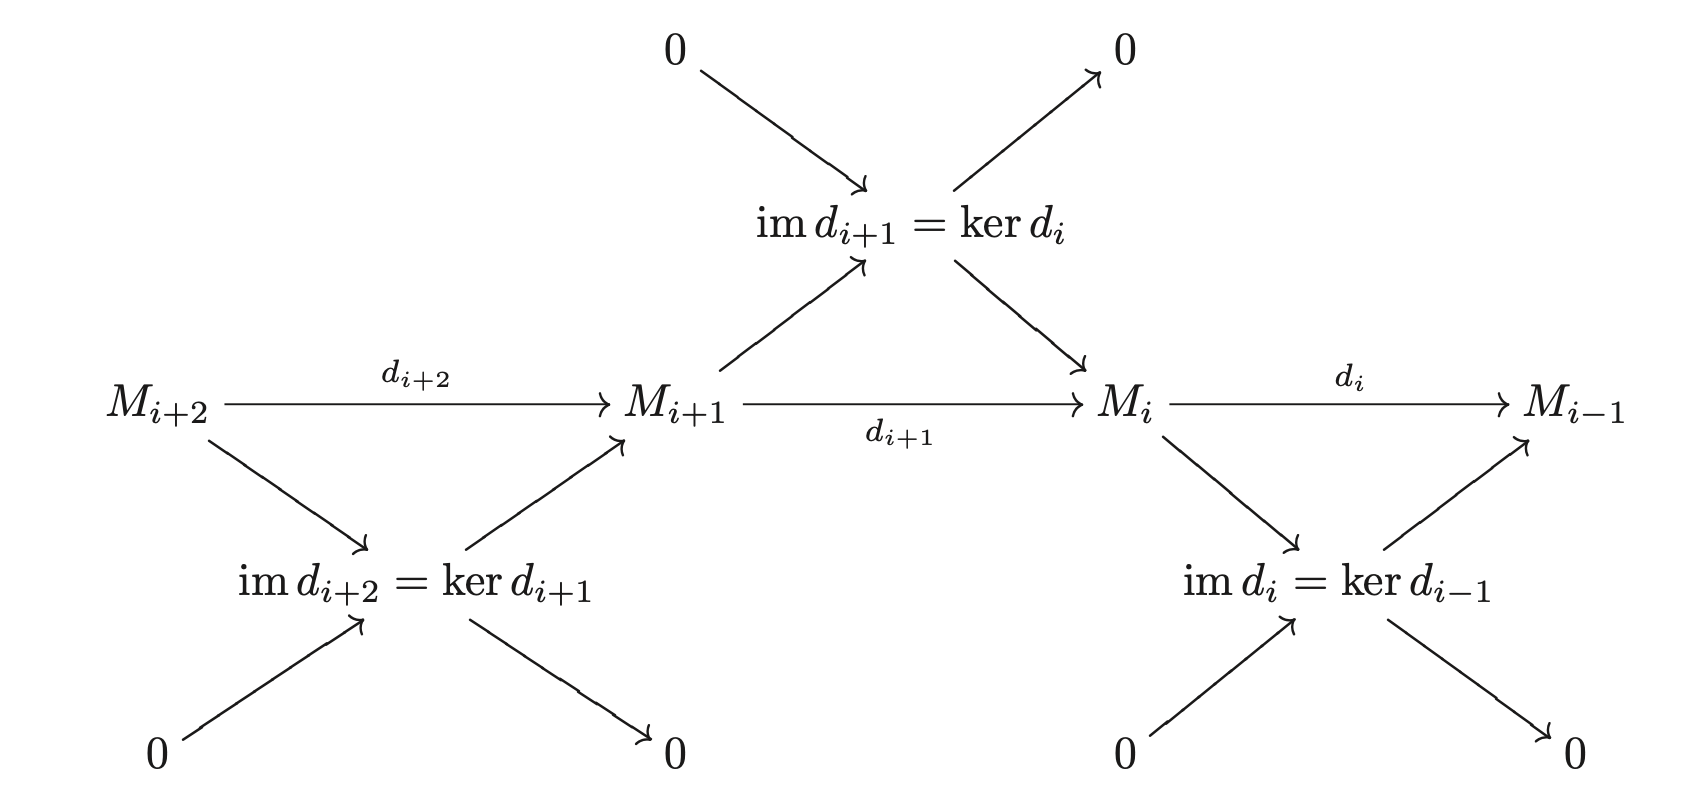
\includegraphics[scale=0.5]{ss.png}
    \end{center}
\end{remark}
Second one is via induction on $n$.
\begin{proof}
    $n=0$ is trivial. Suppose it's true for number less than $n$. Consider the short exact sequence
    \[ 0 \to (0: x_n) \to M(-1) \xrightarrow{x_n} M \to M/x_nM \to 0. \]
    Notice that $M/x_nM$ is a finitely generated graded module over $k[x_1, \ldots, x_{n-1}]$ ($x_n$ acts as zero) and $(0:x_n)$ is also a finitely generated graded module over $k[x_1, \ldots, x_{n-1}]$ (the generators of $(0:x_n)$ over $k[x_1, \ldots, x_{n-1},x_n]$ also generate $(0:x_n)$ over $k[x_1, \ldots, x_{n-1}]$ since $x_n$ would act as zero). By the inductive hypothesis, both $M/x_nM$ and $(0:x_n)$ have Hilbert dimensions agree with polynomials when $d$ is large enough. Thus, by the exactness of the sequence, 
    \[H_M(d)-H_M(d-1)=H_{M/x_nM}(d)-H_{(0:x_n)}(d-1)=\lambda(d).\]
    for some polynomial $\lambda(d)$ when $d$ is large enough.
    Thus, 
    \[H_M(d)-H_M(0) = \sum_{i=1}^d (H_M(i)-H_M(i-1)) = \sum_{i=1}^d \lambda(i).\]
    Notice that $\sum_{i=1}^d i^k$ is a polynomial in $d$ of degree $k+1$. Therefore, $\sum_{i=1}^d \lambda(i)$ is also a polynomial in $d$ when $d$ is large enough.
    Therefore, $H_M(d)$ also agrees with a polynomial when $d$ is large enough. 
\end{proof}

\begin{remark}
    Is $H_M(d)$ always finite? The answer is yes if $M$ is a finitely generated module over $k[x_1, \ldots, x_n]$. This is nontrivial because $H_M(d)$ is considering the dimension of $M$ as module over $k$, not over $R$. 
    \begin{proof}
        Consider $M'=\bigoplus_{s=d}^\infty M_s$. $M'$ is a submodule of $M$, so it's finitely generated as $R$-module. Let $m_1, \ldots, m_t$ be the generators of $M'$. Each $m_i$ has degree at least $d$. So for any element in $M_d$, it's a linear combination of $m_i$ with coefficients in $R$ of degree at most $0$ (otherwise it would have degree greater than $d$). Therefore, $M_d$ is spanned by $m_1, \ldots, m_t$ over $k$, which is finite-dimensional. 
    \end{proof}
    I came up with another more intuitive proof.  
    \begin{proof}
        $M$ is finitely generated as $R$-module by $m_1, \ldots, m_t$. For some degree $d$, any element in $M_d$ must be a linear combination of $m_i$ with coefficients as the monomials in $R$ of degree at most $d-\deg(m_i)$. There are only finitely many such monomials, so $M_d$ is finite-dimensional over $k$.
    \end{proof}
\end{remark}
\newpage 
\section{January 22, 2026: Nullstellensatz and equivalence of affine varieties and affine algebras}
Today we discuss the Hilbert's Nullstellensatz and the equivalence between the category of affine algebraic varieties and the category of finitely generated reduced $k$-algebras. For further details, please refer to \href{https://github.com/AmazingBoBoy/my-website/blob/main/notes/alggeo/note.pdf}{here}. 
\newpage 
\section{January 27, 2026: Localization and Tensor Products}
There is a readiness exam today. 

For problem 3, we have a stronger result. 
\begin{lemma}
For any $R$ and ideals $I$ and $J$, we have an isomorphism
\[\frac{R}{I}\otimes_R \frac{R}{J} \cong \frac{R}{I+J}.\]
\begin{subproof}
    We will show a more general result: 
    For any ideal $I$, we have the exact sequence
    \[ 0 \to I \to R \to R/I \to 0.\]
    Tensoring with $N$, we get the right exact sequence
    \[ I \otimes_R N \to R \otimes_R N \to (R/I) \otimes_R N \to 0.\]
    Notice that the image of $I \otimes_R N$ in $R \otimes_R N \cong N$ is exactly $IN$. Thus, we have the isomorphism $\frac{N}{IN } \cong (R/I) \otimes_R N$. Taking $N=R/J$, we get
    \[ \frac{R/J}{I(R/J)} \cong (R/I) \otimes_R (R/J).\]
    Note that $I(R/J)=IR/J = (I+J)/J$ (an elementary result, informally $I(R/J)$ is just $I/J$, but $I$ may not contain $J$ so we just use $I+J/J$ to avoid confusion), so we have
    \[ \frac{R/J}{I(R/J)} \cong \frac{R}{I+J}.\]
    Combining the two isomorphisms, we get the desired result.
\end{subproof}

\end{lemma}

Next, we discuss localization. We essentially invert elements of a multiplicative subset $U \subseteq R$. 
\begin{proposition}
    Some key properties of localization:
    \begin{enumerate}
    \item There is a natural map $\phi: R \to M[U\inv]$ given by $r \mapsto \frac{r}{1}$. 
    \item For any ideal $J\subseteq R[U\inv]$, $I^c=\phi\inv(I)$ is an ideal of $R$ disjoint from $U$. (This is true in general for any ring homomorphism $\phi$.)
    \item For any ideal $I \subseteq R$ disjoint from $U$, the extension $I^e=U\inv I$ is a proper ideal of $R[U\inv]$. (if they are not disjoint, then $1$ is in the $U\inv I$, so it's not proper). 
    \item For any $J\subseteq R[U\inv]$, we have $J=(J^c)^e$. 
    \item However, the $(I^e)^c\neq I$, even if $I\cap S=\emptyset$. Example: let $U=\{1,x,x^2,\ldots \}$ and $R=\CC[x,y]$, $(xy)^e=(y)$ in $R[U\inv]$ and $((xy)^e)^c= (y)$ in $R$. The correct statement is \[(I^e)^c= \{ r \in R: \exists u \in U, ur \in I\}=\sum_{u\in U} (I:u)\supseteq (I:U)\supseteq I\]. If $I$ is prime, then $(I^e)^c=I$.
    \item This gives us the following bijection of prime ideals between $R$ and $R[U\inv]$: 
    \begin{center}
        \[\begin{tikzcd}[sep=scriptsize]
    {\{\kq \subseteq R[U^{-1}]\}} &&&&&& {\{ \kp\subseteq R:  \kp\cap U=\emptyset\}}
    \arrow["{\phi^{-1}(-)}", curve={height=-24pt}, from=1-1, to=1-7]
    \arrow["{U^{-1}(-)}", curve={height=-24pt}, from=1-7, to=1-1]
\end{tikzcd}\]
    \end{center}
\end{enumerate}
\end{proposition}


\begin{proposition}
    Some key properties of localization as a functor:
    \begin{enumerate}
    \item The universal property of localization: for any $R$-module $M$ and $N$, multiplicative closed set $U$. If $U$ acts invertibly on $N$, then any $R$-module homomorphism $\psi: M \to N$ factors uniquely through $U\inv M$. That is, there exists a unique $R$-module homomorphism $\tilde{\psi}: U\inv M \to N$ such that the following diagram commutes:
    % https://q.uiver.app/#q=WzAsMyxbMCwwLCJNIl0sWzMsMCwiTiJdLFsxLDIsIlVeey0xfU0iXSxbMCwxLCJcXHBzaSJdLFswLDIsIlxccGhpIiwyXSxbMiwxLCJcXHRpbGRle1xccHNpfSIsMl1d
\[\begin{tikzcd}
    M &&& N \\
    \\
    & {U^{-1}M}
    \arrow["\psi", from=1-1, to=1-4]
    \arrow["\phi"', from=1-1, to=3-2]
    \arrow["{\tilde{\psi}}"', from=3-2, to=1-4]
\end{tikzcd}\]
    \item If $R$ is Noetherian, then so is $R[U\inv]$. If $R$ is UFD, then so is $R[U\inv]$.
    \item Localization commutes with direct sums and direct limits because it's a left adjoint functor. It's left adjoint to the forgetful functor from $R[U\inv]$-modules to $R$-modules, forgetting the inverted elements' action. 
    \item Left adjointness implies that localization is right exact. In fact, localization is an exact functor. 
    \item Exactness implies that localization preserves finite limits and finite colimits. In particular, it preserves kernels, cokernels (quotient of modules), finite intersections (intersetctions= a fiber product=a finite limit) and finite products. Left adjointness implies that it preserves colimits (need not to assume finiteness). In general, left exactness preserves finite limits, right exactness preserves finite colimits. 
    \begin{subproof}
        Exactness implies preservation split exact sequences. Thus, this fucntor preserves products and kernels. Any finite limit can be constructed using products and kernels, so it preserves finite limits. Colimit is similar. 
    \end{subproof}
    
    \item Localization is nice with respect to tensor products: 
    Let $M$ and $A$ be $R$-modules, $N$ be an $R[U\inv]$-module, then we have the isomorphism
    \[U\inv R\otimes_R M \cong U\inv M, \]
    \[U\inv (M \otimes_R N)\cong U\inv M\otimes_{U\inv R} N, \]
    \[U\inv(A\otimes_R M)\cong U\inv A\otimes_{U\inv R} U\inv M.\]
    The first isomorphism tells us $(-)\otimes_R U\inv R$ is exact, that is $U\inv R$ is a flat $R$-module.
    \item Tensor products are associative: for any $R$-module $M$, $R$-$S$-bimodule $N$ and $S$-module $P$, we have the isomorphism
    \[(M \otimes_R N) \otimes_S P \cong M \otimes_R (N \otimes_S P).\]
\end{enumerate}
\end{proposition}

 
\begin{proposition}
Properties of tensor products and $\mathrm{Hom}$ functors:
    \begin{enumerate}
    \item $(-)\otimes_R M$ is left adjoint to $\mathrm{Hom}_R(M,-)$. Thus, $\mathrm{Hom}_R(M,-)$ is right exact.    \item $h_N(-)=\mathrm{Hom}_R(-,N): \text{R-Mod}^{\text{op}} \to \text{R-Mod}$ is right adjoint to $h_N(-)^{\text{op}}: \text{R-Mod} \to \text{R-Mod}^{\text{op}}$. 
\end{enumerate}
\end{proposition}

\newpage 
\section{January 29, 2026: More on Localization}
Some multiplicative closed sets that are often used:
\begin{enumerate}
    \item $U=R_x={1,x,x^2,\ldots }$ for some $x \in R$. The localization $R_x$ is often denoted as $R[x\inv]$.
    \item $U=R \setminus \kp$ for some prime ideal $\kp$. $U\inv R$ is often denoted as $R_\kp$ and called the localization of $R$ at $\kp$.
\end{enumerate}
\begin{example}[The Ring of Laurent Polynomials]
    $k[x]_x=k[x, x\inv]$. 
\end{example}
\begin{example}
    The regular function on an affine open subset $D(f)$ of an affine variety $X$ is given by the localization of the coordinate ring $A(X)$ at $f$, that is $A(X)_f$.
\end{example}
\begin{example}[stalk of a variety at a point]
    Let $X \subseteq \mathbb{A}^n$ be an affine variety over an algebraically closed field $k$. For any point $p \in X$, the stalk of $X$ at $p$ (all regular functions that are well-defined locally at $p$) is isomorphic to the localization of the coordinate ring $A(X)$ at the maximal ideal $\km_p$ corresponding to the point $p$. That is, 
    \[\mathcal{O}_{X,p}=A(X)_{\km_p}=\{\frac{f}{g} \mid f,g \in A(X), g(p)\neq 0\}. \]
    
\end{example}
\begin{example}
    $(\ZZ/10\ZZ)_2 \cong \ZZ/5\ZZ$.
    \begin{proof}
        $(\ZZ/(10))_2=(\ZZ_2/(10)_2)=(\ZZ_2/(5)_2)=(\ZZ/(5))_2=\ZZ/5\ZZ$. 
        \\
        Most equalities are guaranteed by the fact that localization preserves quotients. The last step is because $\ZZ/(5)$ is a field, so any nonzero element is invertible.
    \end{proof}
\end{example}
\begin{theorem}[Local Global Principle]
    $M=0$ if and only if $M_\kp=0$ for all prime ideals $\kp$ if and only if $M_\km=0$ for all maximal ideals $\km$.
\end{theorem}
\begin{remark}
    One way to understand this theorem is through dimension argument in algebraic geometry. The codimension of a point (the largest dimension of objects containing the point) is the same as the height of the corresponding prime ideal, which is the Krull dimension of the localized ring at that prime ideal. If the codimenson of any point is $0$, then the variety is empty! So the coordinate ring of the variety is $0$. 
    \\

    Another way to understand this theorem is through the stalks of a sheaf. If a ring of regular functions is $0$ at every stalk (the small neighborhood of every point), then the only function in the ring is the zero function. So the ring itself is $0$.
\end{remark}
\begin{theorem}
    A sequence of $R$-modules is exact if and only if the localized sequence at any prime ideal is exact if and only if the localized sequence at any maximal ideal is exact. 
    \\

    In particular, an $R$-module homomorphism $\phi: M \to N$ is injective (surjective) if and only if the localized homomorphism $\phi_\kp: M_\kp \to N_\kp$ is injective (surjective) for all prime ideals $\kp$ if and only if the localized homomorphism $\phi_\km: M_\km \to N_\km$ is injective (surjective) for all maximal ideals $\km$.
\end{theorem}

\begin{example}[Chinese Remainder Theorem]
    Let $R$ be a ring, and let $Q_i$ be ideals of $R$ such that $Q_i+Q_j=R$ for all $i \neq j$. Then we have the isomorphism
    \[R/\bigcap_{i=1}^n Q_i \cong \bigoplus_{i=1}^n R/Q_i.\]
    Furthermore, one can show that $\bigcap_{i=1}^n Q_i = \prod_{i=1}^n Q_i$.
    \begin{subproof}
        We have a natural injection from $R/\bigcap_{i=1}^n Q_i$ to $\bigoplus_{i=1}^n R/Q_i$ given by $r \mapsto (r+Q_1, \ldots, r+Q_n)$. We will show that this map is also surjective by localization.
        \\
        For any maximal ideal $\km$ of $R$, there is at most one $Q_i$ contained in $\km$ since $Q_i+Q_j=R$ for all $i \neq j$. Since $Q_j$ is not contained in $\km$, then the localization of $Q_j$ at $\km$ is the whole localized ring $R_\km$.
        \\

        When we localize the injection at $\km$, we get the map 
        \[R_{\km}/\bigcap_{i=1}^n (Q_i)_{\km} \to \bigoplus_{i=1}^n R_{\km}/(Q_i)_{\km}.\]
        That is, 
        \[R_{\km}/(Q_i)_{\km} \to R_{\km}/(Q_i)_{\km}.\]
        which is clearly an isomorphism. Thus, the localized map is an isomorphism for any maximal ideal $\km$. By the local global principle, the original map is also an isomorphism.
    \end{subproof}
\end{example}
\begin{theorem}
    Let $R$ be a ring, and $S$ be a $R$-algebra and $S$ is flat as an $R$-module. If $M$ and $N$ are $S$-modules, and $M$ is finitely presented as an $R$-module, then we have the isomorphism
\[S\otimes_R\mathrm{Hom}_R(M,N) \cong \mathrm{Hom}_S(M\otimes_R S,N\otimes_R S).\]

\end{theorem}
\begin{proof}
    There is a natural homomorphism \[\alpha_M: S\otimes_R\mathrm{Hom}_R(M,N) \to \mathrm{Hom}_S(M\otimes_R S,N\otimes_R S)\] sending $s\otimes f$ to the homomorphism $m\otimes s' \mapsto f(m)\otimes ss'$. 
    \\

    First, if $M$ is a free $R$-module, then $\alpha$ is an isomorphism, this is very easy. Thus, for any finitely presented $R$-module $M$, we have an exact sequence 
    \[F\to G\to M \to 0.\]
    where $F$ and $G$ are free $R$-modules. Applying $\hom_R(-, N)$, we get the exact sequence
    \[0 \to \mathrm{Hom}_R(M,N) \to \mathrm{Hom}_R(G,N) \to \mathrm{Hom}_R(F,N).\]
    Applying $S\otimes_R -$ ($S$ is flat), we get the exact sequence
    \[0 \to S\otimes_R\mathrm{Hom}_R(M,N) \to S\otimes_R\mathrm{Hom}_R(G,N) \to S\otimes_R\mathrm{Hom}_R(F,N).\]
    On the other hand, applying $-\otimes_R S$ to the first exact sequence, we get the exact sequence
    \[F\otimes_R S \to G\otimes_R S \to M\otimes_R S \to 0.\]
    Applying $\mathrm{Hom}_S(-,N\otimes_R S)$, we get the exact sequence
    \[0 \to \mathrm{Hom}_S(M\otimes_R S,N\otimes_R S) \to \mathrm{Hom}_S(G\otimes_R S,N\otimes_R S) \to \mathrm{Hom}_S(F\otimes_R S,N\otimes_R S).\]
    We have the following commutative diagram:
    \[\begin{tikzcd}
    0 && 0 \\
    0 && 0 \\
    S\otimes_R\mathrm{Hom}_R(M,N) && \mathrm{Hom}_S(M\otimes_R S,N\otimes_R S) \\
    S\otimes_R\mathrm{Hom}_R(G,N) && \mathrm{Hom}_S(G\otimes_R S,N\otimes_R S) \\
    S\otimes_R\mathrm{Hom}_R(F,N) && \mathrm{Hom}_S(F\otimes_R S,N\otimes_R S)
    \arrow[from=1-1, to=2-1]
    \arrow[from=1-3, to=2-3]
    \arrow["0", from=1-1, to=1-3]
    \arrow["0", from=2-1, to=2-3]
    \arrow["\alpha_M", from=3-1, to=3-3]
    \arrow["\alpha_G", from=4-1, to=4-3]
    \arrow["\alpha_F", from=5-1, to=5-3]
    \arrow[from=2-1, to=3-1]
    \arrow[from=3-1, to=4-1]
    \arrow[from=2-3, to=3-3]
    \arrow[from=3-3, to=4-3]
    \arrow[from=4-1, to=5-1]
    \arrow[from=4-3, to=5-3]
\end{tikzcd}\]
By five lemma, $\alpha_M$ is an isomorphism.
    
\end{proof}
\begin{application}[Eisenbud's Exercise 2.13]
    If $C$ is finitely presented, then the short exact sequence
    \[0\to A \to B \to C\to 0\]
    splits if and only if 
    
    \[0\to A_p \to B_p \to C_p \to 0\]
    splits for all prime ideals $p$.
    \\
    
    The key idea is to use the facts: $R_p$ is flat and 
    \[0\to A \to B \to C\to 0\]
    splits if and only if  \[0\to \hom(C,A) \to \hom(C,B) \to \hom(C,C) \to 0\] is exact.
\end{application}

\begin{theorem}
    \[\sqrt{I}=\bigcap_{\kp \supseteq I} \kp\]
\end{theorem}
\begin{proof}
    One direction is trivial. For the nontrivial one, assume $f\in \kp$ for all prime ideals $\kp$ containing $I$. We want to show that $f \in \sqrt{I}$. If not, then we can localize at $\{|f^n: n \geq 0\}$. In the localized ring, $I_f$ is a proper ideal, so there exists a maximal ideal $\km$ containing $I_f$. $\km$ corresponds to a prime ideal $\kp$ in the original ring containing $I$ but not containing $f$, contradicting the assumption.
\end{proof}
\newpage 
\section{February 3, 2026: Finite Length and Artinian}
Today we discuss the finite length condition. 

\begin{definition}
    We define the length of a module $M$ to be the smallest integer $\ell(M)=n$ such that there exists a chain of submodules of $M$ of length $n$:
\[M=M_0\supsetneq M_1 \supsetneq \cdots \supsetneq M_n=0.\]
If such $n$ does not exist, we say $M$ has infinite length. If $M$ has finite length, we say $M$ is of finite length.
\end{definition}
\begin{lemma}
    Let $N$ be a simple $R$-module, then $N \cong R/\km$ for some maximal ideal $\km$ of $R$. In fact, $\km=\Ann(N)$.
\end{lemma}
\subsection{Main theorems of finite length modules and rings}
\begin{theorem}
    Let $R$ be a ring, and $M$ be an $R$-module. $M$ has a finite composition series if and only if $M$ is both Noetherian and Artinian. If $M=M_0\supsetneq M_1 \supsetneq \cdots \supsetneq M_n=0$ has a finite composition series, then 
    \begin{enumerate}
        \item Any strictly descending chain of submodules of $M$ has length at most $n$.
        \item Any composition series of $M$ has length $n$. This gives a well-defined notion of the length of $M$, denoted as $\ell(M)$, which is the length of any composition series of $M$.
        \item The sum of localization maps $M\to M_{\km}$ for all maximal ideals $\km$ gives an isomorphism of $R$-modules: 
        \[M\cong \bigoplus_{\km} M_{\km}\]
        where the sum is take over all maximal $\km$ such that $\frac{M_i}{M_{i+1}} \cong R/\km$ for some $i$. Note that for each maximal ideal $\km$, we only use it once even if it appears multiple times as composition factors.
        \item The number of composition factors isomorphic to $R/\km$ is the same as the length of $M_{\km}$ as $R_{\km}$-module. Thus, it's indepenent of the choice of composition series. Furthermore, any two composition series of $M$ have the same multiset of composition factors. 
        \item $M=M_{\km}$ if and only if $M$ is annihilated by some power of $\km$. 
        \item For any submodule $N\subseteq M$, $\ell(M)=\ell(N)+\ell(\frac{M}{N})$. And the composition factors of $M$ is the disjoint union of the composition factors of $N$ and $M/N$ as multisets.
    \end{enumerate}
\end{theorem}
\begin{proof}
    If $M$ is Artinian and Noetherian, we can pick a maximal proper submodule $M_1$ of $M$ (by Noetherian condition), then $M/M_1$ is simple. Then, we pick a maximal proper submodule $M_2$ of $M_1$, and so on. We can continue this process to get a composition series. It must be finite because $M$ is Artinian.
    \\
    
    First, show that if $M'$ is a proper submodule of $M$, then $\ell(M')<\ell(M)$, that is for any composition series of $M$ of length $n$, we can find a composition series of $M'$ of length less than $n$. Just take the intersection of $M'$ with the composition series of $M$.
    This would give us $M'\supseteq M'\cap M_1 \supseteq M' \cap M_2 \supseteq \cdots \supseteq M' \cap M_n=0$. We claim that this is a composition series of $M'$. Notice that $\frac{M'\cap M_i}{M' \cap M_{i+1}}\cong \frac{M'\cap M_i+M_{i+1}}{M_{i+1}}\subseteq \frac{M_i}{M_{i+1}}$ is either $0$ or $\frac{M_i}{M_{i+1}}$ which are btoh simple. And it can't be $\frac{M_i}{M_{i+1}}$: if $M'\cap M_i+M_{i+1}=M_i$ for all $i$, $M' \supseteq M_i$ for all $i$ (induct from $i=n$ to $i=0$), so $M'=M$, contradiction. Thus, we have $\ell(M')<\ell(M)$.
    \\

    Second, we show that for any strictly descending chain of submodules of $M$, its length is at most $\ell(M)$. We proceed by induction on $\ell(M)$. If $\ell(M)=0$, trivial. If $\ell(M)=n$, we have $M=M_0\supsetneq N_1 \supsetneq \cdots \supsetneq N_k=0$. Notice $N_1$ is a proper submodule of $M$, so $\ell(N_1)<\ell(M)=n$. By the inductive hypothesis, $k-1 \leq \ell(N_1)<n$. Thus, $k \leq n$.
    \\

    Third, we can show that any composition series of $M$ has length $n$. For any $M=M_0\supsetneq M_1 \supsetneq \cdots \supsetneq M_n=0$ is a composition series of $M$. By the definiton of $\ell(M)$, we have $\ell(M)\leq n$. On the other hand, by what we just proved, any strictly descending chain of submodules of $M$ has length at most $\ell(M)$, so $n \leq \ell(M)$. Thus, $n=\ell(M)$. So all composition series of $M$ have the same length, which is $\ell(M)$.
    \\

    Fourth, we can show that $M$ is Noetherian and Artinian. For any ascending chain of submodules of $M$, its length is at most $\ell(M)$, so it must stabilize. For any descending chain of submodules of $M$, its length is at most $\ell(M)$, so it must stabilize. 
    \\

    Fifth, we want to show (3). It suffices to show the isomorphism when we localize at any maximal ideal $Q$. We begin with the case when $\ell(M)=1$, that is, when $M$ is simple. $M\cong R/\km$ for some maximal ideal $\km$. If $\km=Q$, then $M_Q\cong (\frac{R}{Q})_Q$. Since $\frac{R}{Q}$ is a field, any nonzero element is invertible, so $(\frac{R}{Q})_Q \cong \frac{R}{Q}$. If $\km \neq Q$, then $M_Q\cong (\frac{R}{\km})_Q=0$ since $\km$ becomes the whole ring after localization. In particular, we conclude that if $Q$ and $Q'$ are two different maximal ideals and $M$ is a simple module, then $(M_Q)_{Q'}=0$.
    \\
    
    Sixth, we now return to the general case. Let $M$ be an $R$-module of length $n$. We have a composition series of $M$:
    \[M=M_0\supsetneq M_1 \supsetneq \cdots \supsetneq M_n=0.\]
    We can localization at any maximal ideal $Q$ to get the series of $M_Q$:
    \[M_Q=(M_0)_Q\supseteq (M_1)_Q \supseteq \cdots \supseteq (M_n)_Q=0.\]
    Notice that $\frac{(M_i)_Q}{(M_{i+1})_Q}\cong (\frac{M_i}{M_{i+1}})_Q$ is either $0$ or $\frac{M_i}{M_{i+1}}$. So this is a composition series of $M_Q$ (some terms may be repeated). We denote $\frac{M_i}{M_{i+1}} \cong R/\km_i$. If $\km_i=Q$, then $\frac{(M_i)_Q}{(M_{i+1})_Q}\cong R/Q$. If $\km_i \neq Q$, then $\frac{(M_i)_Q}{(M_{i+1})_Q}=0$. Thus, the length of $M_Q$ is the number of composition factors of $M$ isomorphic to $R/Q$. This tells us the compistion factors of $M$ is indepenent from the choice of composition series, and any two composition series of $M$ have the same multiset of composition factors. In particular, if there is no composition factor of $M$ isomorphic to $R/Q$, then $M_Q=0$. 
    Furthermore, $(M_Q)_{Q'}=0$ for any two distinct maximal ideals $Q$ and $Q'$. 
    \\

    Seventh, consider $\phi: M \to \bigoplus_{\km} M_{\km}$ where $\km$ runs through all maximal ideals corresponding to the composition factors of $M$. Since $M_Q=0$ for any maximal ideal $Q$ that is not corresponding to the composition factors of $M$, we can harmlessly extend the sum to all maximal ideals of $R$. We will show that $\phi$ is an isomorphism.
    \\

    For any maximal ideal $Q$, we have 
    \[\phi_Q: M_Q\to M_Q\]
    Since $(M_Q)_{Q'}=0$ for any two distinct maximal ideals $Q$ and $Q'$, the localization of $\bigoplus_{\km} M_{\km}$ at $Q$ is just $M_Q$. Thus, $\phi_Q$ is an isomorphism. By the local global principle, $\phi$ is an isomorphism.
    \\

    Eighth, we let $M=\oplus_{\km_i} M_{\km_i}$. If $M$ is annihilated by some power of $\km$, then we claim that $M=M_{\km}$. If not, then there exists some maximal ideal $\km_j \neq \km$ such that $M_{\km'}\neq 0$. Therefore, there exists $a\in \km$ but $a\notin \km_j$. Since $M_{\km_j}$ is annihilated by some power of $\km$, there exists some $n$ such that $a^n M_{\km_j}=0$. On the other hand, since $a\notin \km_j$, $a$ is invertible in $R_{\km_j}$, so $M_{\km_j}=0$, contradiction. Thus, we have $M=M_{\km}$. Conversely, if $M=M_{\km}$, then the compistion factors of $M$ are all isomorphic to $R/\km$, so $M$ is annihilated by some power of $\km$.
    \\

    Lastly, combining the composition series of $N$ and $M/N$, we can get a composition series of $M$. Thus, $\ell(M)=\ell(N)+\ell(M/N)$. In particular, if $N$ and $M/N$ are of finite length, then so is $M$. Conversely, we can always construct a composition series of $M$ containing $N$ to get a compistion series of $N$ and $M/N$. Therefore, the disjoint union of their compistion factors is the composition factors of $M$ as multisets.
\end{proof}
\begin{remark}
    Notice that $M\cong \bigoplus_{\km} M_{\km}$. This is direct sum. \textbf{NOT} direct product. And the proof doesn't work with infinite direct product because localization is left adjoint, so it preserves colimits but not limits. 
\end{remark}
\begin{theorem}
    Let $R$ be a ring. The following are equivalent:
    \begin{enumerate}
        \item $R$ is of finite length as an $R$-module.
        \item $R$ is Artinian.
        \item $R$ is Noetherian and has Krull dimension $0$ (that is, all prime ideals of $R$ are maximal).
    \end{enumerate}
    If that's the case, then there are finitely many prime ideals=maximal ideals of $R$. 
\end{theorem}
\begin{proof}
    (1) to (2) is proven by the previous proposition. 
    \\

    (2) to (3): 
    \begin{claim}
    $0$ is the product of finitely many maximal ideals.
    \begin{subproof}
        Let $\SF$ the be family of all ideals that are product of finitely many maximal ideals (can be repeated). $\SF$ is clearly nonempty, thus by Artinian condition, there is a minimal element in $\SF$, say $J$.
        \\
        By the maximality of $J$, for any maximal ideal $\km$, $J\km=J$ and $J\subseteq M$. We also have $J^2\subseteq J$, so $J^2=J$. 
        \\

        We claim that $J=0$. If not, let $\SF'$ be the family of all ideals $I$ such that $IJ\neq 0$. Let $I$ be the minimal element of $\SF'$. Thus, $IJ=IJ^2=(IJ)J$. Thus, $IJ=I$ by the minimality of $I$. So there must exists $f\in I$ such that $(f)J\neq 0$. So $I=(f)$. So $(f)J=(f)$. Thus, there eixsts $g\in J$ such that $fg=f$. So $f(1-g)=0$. Since $J$ is contiained in all maximal ideals, $1-g$ is not contained in any maximal ideals, so $1-g$ is invertible. Thus, $f=0$, contradiction. So $J=0$.
    \end{subproof} 
    \end{claim}
    

    Thus, we have $0=\km_1\cdots \km_n$ for some maximal ideals $\km_1, \ldots, \km_n$. This implies that for any prime ideal $\kp$, $\kp\subseteq (0)=\km_1\cdots \km_n \subseteq \km_i$ for some $i$. We claim that $\kp\supseteq \km_i$. If not, there eixsts $f_i\in \km_i$ but $f_i\notin \kp$ for all $i$. But $\prod_{i=1}^n f_i \in \km_1\cdots \km_n =0 \subseteq \kp$, so at least one $f_i\in \kp$. Thus, $\kp\supseteq \km_i$ is maximal. Therefore, any prime ideal of $R$ is maximal and there are only finitely many prime ideals of $R$.
    \\

    We now show that $R$ is Noetherian. Consider $M_i=\frac{\km_1\cdots \km_i}{\km_1\cdots \km_i\km_{i+1}}$ as $R/\km_{i+1}$-vector spaces. 
    \begin{claim}
        $M_i$ is finite-dimensional as $R/\km_{i+1}$-vector space.
        \begin{subproof}
        For any subspace of $M_i$, it corresponds to an ideal $I\subseteq R$. Since $R$ is Artinian, any descending chain of subspaces of $M_i$ must stabilize, so $M_i$ is finite-dimensional. Thus, we can construct a $M_i\supseteq M_{i,1} \supseteq \cdots \supseteq M_{i,n_i}=0$ such that $M_{i,j}/M_{i,j+1}\cong R/\km_{i+1}$ for all $j$. This is a finite composition series of $M_i$ as $R$-module, so $M_i$ is of finite length as $R$-module. Putting the composition series of $M_i$ together, we can get a composition series of $R$. Thus, by the previous proposition, $R$ is Noetherian.
    \end{subproof}
    \end{claim}
    
    (3) to (1): Assume $R$ is not of finite length. Consider $\SF$ to be the family of ideals such that $R/I$ is not of finite length as $R$-module. $\SF$ is clearly nonemtpy since $(0) \in \SF$, so there is a maximal element $I$ in $\SF$. 
    \begin{claim}
        $I$ is a prime ideal. 
        \begin{subproof}
        if not, then there exisst $ab\in I$ but $a,b\notin I$. Thus, $(I:a) \supsetneq I$ and $(I)+(a) \supsetneq I$. Thus, $\frac{R}{(I:a)}$ and $\frac{R}{I+(a)}$ are both of fintie length. Consider the exact sequence of $R$-modules: 
        \[0 \to \frac{R}{(I:a)} \taking{\times a} \frac{R}{I} \to \frac{R}{I+(a)} \to 0.\]
        Pasting the composition series of $\frac{R}{(I:a)}$ and $\frac{R}{I+(a)}$, we can get a finite composition series of $\frac{R}{I}$, so $\frac{R}{I}$ is of finite length, contradiction. Thus, $I$ is a prime ideal.
        \\

        Since $I$ is also maximal ideal. $R/I$ is a field, so $R/I$ is of finite length, contradiction. Thus, $\SF$ is empty and $R$ is of finite length.
    \end{subproof}
    \end{claim}
    
    Finally, we complete the proof. 
\end{proof}
With two main theorems, we can state the following corollary regarding the properties of Artinian rings and modules of finite length.
\begin{corollary}
    Here are a few properties of Artinian rings:
    \begin{enumerate}
        \item Any quotient of an Artinian ring is Artinian. 
        \item Any localization of an Artinian ring is an Artinian ring.
    \end{enumerate}
    In module theory, we have the following properties of module of finite length (or Artinian if we assume it's finitely generated module over a Noetherian ring):
    \begin{enumerate}
        \item Any submodule of finite length module is of finite length.
        \item Any quotient of finite length module is of finite length.
        \item Any localization of finite length module is of finite length 
        \\($U\inv\frac{M_i}{M_{i+1}}\cong U\inv R/\km_i\cong \frac{U\inv R}{U\inv \km_i}=0$ or a simple module).
    \end{enumerate}
\end{corollary}

Now, we put this in a geometric setting: 
\begin{theorem}
    Let $X$ be an affine variety over an algebraically closed field $k$. The following are equivalent:
    \begin{enumerate}
        \item $X$ is a finite set of points. 
        \item $A(X)$ is a finite-dimensional $k$-vector space, and its dimension is exactly the number of points in $X$.
        \item $A(X)$ is Artinian. 
    \end{enumerate}
\end{theorem}
\begin{proof}
    (1) to (2): Let $p_i$ be the points in $X$. They are disconnected, so $A(X)=\prod_{p_i\in X}A(p_i)=k^n$ where $n$ is the number of points in $X$.
    \\

    (2) to (3): If $A(X)$ is a finite-dimensional $k$-vector space, then it has a finite composition series as $A(X)$-module, so it's Artinian. Or, any descending chain of ideals of $A(X)$ is also a descending chain of subspaces of $A(X)$, so it must stabilize since the dimension of $A(X)$ is finite. 
    \\

    (3) to (1): If $A(X)$ is Artinian, then $A(X)$ has finitely many prime ideals, which are all maximal. Thus, $X$ has finitely many points.
\end{proof}

\begin{theorem}[Structure Theorem for Artinian Rings]
    Let $R$ be an Artinian ring, which is also module of finite length as $R$-module. Then we have the isomorphism
    \[R\cong \bigoplus_{i=1}^n R_{\km_i}\]
    where each $R_{\km_i}$ is an Artinian local ring.
\end{theorem}
\begin{proof}
    The isomorphism we had for $R$ as $R$-module is actually an isomorphism of rings. The ring structure on $\bigoplus_{i=1}^n R_{\km_i}$ is given by the componentwise multiplication. Beyond that, we need to show the localization of an Artinian ring is Artinian. This is because the localization of an Artinian ring must be Noetherian. Prime ideals of the localized ring correspond to prime ideals of the original ring contained in the maximal ideal we localize at. So in fact, the localized ring has only one prime ideal, which is maximal, so it has Krull dimension $0$. Thus, the localized ring is Artinian.
\end{proof}
\subsection{Some special cases}
In reality, we are mainly interested in the case when $R$ is Noetherian and $M$ is finitely generated. In this case, we have the following corollary:
\begin{corollary}
    Let $R$ be a Noetherian ring, and let $M$ be a finitely generated $R$-module. The following are equivalent:
    \begin{enumerate}
        \item $M$ is of finite length as $R$-module.
        \item Some finite product of maximal ideals of $R$ annihilates $M$. (can be repeated)
        \item All primes that contain $\Ann(M)$ are maximal ideals
        \item $R/\Ann(M)$ is Artinian.
        \item $M$ is Artinian. 
    \end{enumerate}
\end{corollary}
\begin{proof}
    (1) to (2): Trivial. 
    \\
    (2) to (3): if a prime ideal $\kp$ contains $\Ann(M)\supseteq \km_1\cdots \km_n$, then $\kp$ contains some $\km_i$, which is a maximal ideal. Thus, $\kp$ is a maximal ideal.
    \\
    (3) to (4): Trivial. 
    \\
    (4) to (1): Let $S=\frac{R}{\Ann(M)}$. Since $S$ is Artinian, $S$ is of finite length as $S$-module. $M$ is finitely generated as $R$-module, we claim that $M$ is also finitely generated as $S$-module: $\phi: R^n\surjto M$, we can define a map from $S^n$ to $M$ by sending $r_1+\Ann(M), \ldots, r_n+\Ann(M)$ to $\phi(r_1, \ldots, r_n)$. This is well-defined since $\phi(\Ann(M)^n)=0$ and clearly surjective. Thus, $M$ is a quotient of $S^n$. So $M$ is of finite length as $S$-module, so it's also of finite length as $R$-module since any composition factor in $S$-module is also simple as $R$-module.
    \\
    (1) is equivalent to (5) is proven by the previous proposition.
\end{proof}
\begin{corollary}
    Let $R$ be a Noetherian ring, and let $M$ be a finitely generated $R$-module, $I=\Ann(M)$. Then $M_{\kp}$ is of finite length as $R_{\kp}$-module if and only if $\kp$ is a minimal prime of $I$.
    \\

    This gives us a way to make a module into a module of finite length by localizing at the minimal primes of its annihilator. It also gives us a way to detect the minimal primes of an ideal $I$ by letting $M=R/I$. We will see this in the next corollary.
\end{corollary}


\begin{proof}

First, we need a lemma: 
\begin{lemma}
        If $M$ is finitely generated $R$-module, then $\Ann_{U\inv R}(U\inv M)\cong U\inv \Ann_{R}(M)$ as $U\inv R$-modules. 
        \\

        This is not ture if $M$ is not finitely generated: take $R=\ZZ$, $M=\frac{\QQ}{\ZZ}$ and $U=\ZZ^\times$, $\Ann(M)=0$ but $U\inv M=0$ so $\Ann(U\inv M)=\QQ$. 
    \end{lemma}
       

    By the corollary above, we know that $M_{\kp}$ is of finite length as $R_{\kp}$-module if and only if $R_{\kp}/\Ann(M_{\kp})$ is Artinian. By the lemma, this is equivalent to $R_{\kp}/I_{\kp}$ is Artinian.
   If $\kp$ is a minimal prime of $I$, then $\kp_{\kp}$ is the minimal prime of $I_{\kp}$ as well as the only maximal prime of $R_{\kp}$, so it is the only prime of $R_{\kp}$ containing $I_{\kp}$. Thus, $R_{\kp}/I_{\kp}$ is Artinian. 
   \\
   
   Conversely, if $R_{\kp}/I_{\kp}$ is Artinian, then all primes of $R_{\kp}$ containing $I_{\kp}$ are maximal. But $R_{\kp}$ is a local ring with a unique maximal ideal $\kp_{\kp}$, so $\kp_{\kp}$ is the only prime of $R_{\kp}$ containing $I_{\kp}$. So when we delocalize, we can see that $\kp$ is the only prime of $R$ containing $I$ that is contained in $\kp$, so $\kp$ is a minimal prime of $I$.
\end{proof}
We can let $M=R/I$ in the previous corollary to get the following result about ideals of Noetherian rings and minimal primes of ideals.
\begin{corollary}
    Let $I$ be an ideal of a Noetherian ring $R$ and $\kp$ is a prime containing $I$.  Then the following are equivalent:
    \begin{enumerate}
        \item $\kp$ is a minimal prime of $I$.
        \item There exists $n$ such that $\kp_{\kp}^n \subseteq I_{\kp}$, that is $\kp_{\kp}$ is nilpotent in $R_{\kp}/I_{\kp}$.
        \item $R_{\kp}/I_{\kp}=(R/I)_{\kp}$ is Artinian/finite length as $R_{\kp}$-module.
    \end{enumerate}
\end{corollary}
The idea of the proof is the same as the previous corollary.

\newpage 
\section{February 5, 2026: Associated Primes}
Chapter 3 of Eisenbud's book is about associated primes. It's absolutely horrible and messy in my opinion. I will try to give a more clean and organized presentation of the material in this chapter.
\begin{lemma}
    $I$ is an annihilator of some nonzero element $m$ of $M$ if and only if $R/I$ can be embedded into $M$ as $R$-module. $R/I\cong (m)\subseteq M$. 
\end{lemma}
\subsection{The main theorem about associated primes including filtration and orthogonal lemma}
\begin{theorem}
    This is the main result of today: Let $R$ be a Noetherian ring, and $M$ be a finitely generated $R$-module. Then, 
    \begin{enumerate}
        \item $\Ass(M)$ is nonempty
        \item $\Ass(M)$ is finite
        \item The union of all associated primes of $M$ is exactly the union of all annihilators of nonzero elements of $M$. In particular, if $M=R$, then the union of all associated primes of $R$ is exactly the set of zero-divisors of $R$.
        \item $\Ass_{U\inv R}(U\inv M)=\{U\inv \kp: \kp \in \Ass_R(M), \kp \cap U = \emptyset\}$. 
        \item All the minimal primes of $\Ann(M)$ are in $\Ass(M)$. 
    \end{enumerate}
\end{theorem}
\begin{proof}
    (1): Since $M$ is Noetherian, we can pick the maximal element $I$ in the family of annihilators of nonzero elements of $M$. Say $I=\Ann(m)$ for some $m\neq 0$. We claim that $I$ is a prime ideal. For any $ab\in I$, we have $abm=0$. If $a\notin I$,  Notice that $\Ann(m)\subseteq \Ann(am)$. By the maximality of $I$, we have $\Ann(m)=\Ann(am)$. Thus, $b\in \Ann(am)=I$. So $I$ is a prime ideal, and $I\in \Ass(M)$.
    \\

    We can in fact show a stronger result, for any nonzero element $m\in M$, there exists some associated prime $\kp$ of $M$ such that $\Ann(m)\subseteq \kp$. This is because we can pick the maximal element $I$ in the family of annihilators of nonzero elements of $M$ that contains $\Ann(m)$. By the same argument as above, $I$ is a prime ideal, so $I\in \Ass(M)$ and $\Ann(m)\subseteq I$.
    \\

    (2): we first need to introduce filtration of $M$. 
    \begin{lemma}
        If $R$ is Noetherian and $M$ is a finitely generated $R$-module, then there exists a filtration of $M$:
        \[0=M_0\subsetneq M_1 \subsetneq \cdots \subsetneq M_n=M\]
        such that $M_i/M_{i-1}\cong R/\kp_i$ for some prime ideal $\kp_i$ of $R$.
        \begin{subproof}
        Notice that $\Ass(M)$ is nonempty, so we can pick $\kp_1\in \Ass(M)$ such that there exist $R/\kp_1\cong M_1\subseteq M$. Then we can consider $M/M_1$, which is also a finitely generated $R$-module, so we can pick $\kp_2\in \Ass(M/M_1)$ such that there exist $R/\kp_2\cong M_2/M_1\subseteq M/M_1$. Thus, we get an ascending chain of submodules of $M$:
        \[0=M_0\subsetneq M_1 \subsetneq M_2 \cdots\]
        By Noetherian condition, this chain must stabilize, so we can get a filtration of $M$ as desired.
    \end{subproof}
    \end{lemma}
    
    \begin{lemma}[Orthogonal lemma]
        If $\kp=\Ann(m)$ for some $m\in M$, then $\kp=\Ann(m')$ for all nonzero $m'\in (m)$. 
        \\

        Furthermore, if $R/\kp_1\cong (m_1)\subseteq M$ and $R/\kp_2\cong (m_2)\subseteq M$, then either $\kp_1=\kp_2$ or $(m_1)\cap (m_2)=0$. In other words, each associated primes correspond to cyclic submodules of $M$ that are orthogonal to each other.
        \begin{subproof}
        The first one is easy. The second follows immediately from the first one: if there exists some nonzero element in $(m_1)\cap (m_2)$, then its annihilator is both $\kp_1$ and $\kp_2$, so $\kp_1=\kp_2$.
    \end{subproof}
    \end{lemma}
    
    \begin{lemma}
        All associated primes $\kp$ of $M$ appear in the filtration of $M$ we just constructed. 
        \begin{subproof}
        Let $\kp$ be an associated prime of $M$ and $N\subseteq M$ be a cyclic submodule such that $N\cong R/\kp$. We have shown that either $\kp=\kp_1$ or $N\cap M_1=0$. For the latter case, we can consider $N\cong \frac{N+M_1}{M_1}\subseteq \frac{M}{M_1}$. We can apply the same argument to $N$ and $M_2/M_1$, and so on. Eventually, we must have $\kp=\kp_i$ for some $i$.
    \end{subproof}
    \end{lemma}
    
    with this lemma, we can show that $\Ass(M)$ is finite since there are only finitely many $\kp_i$ in the filtration of $M$.
    \\

    (3): For any nonzero element $m\in M$, we can find the maximal element $I$ in the family of annihilators of nonzero elements of $M$ that contains $\Ann(m)$. This, we conclude that the union of all associated primes of $M$ is exactly the union of all annihilators of nonzero elements of $M$. In particular, if $M=R$, then the union of all associated primes of $R$ is exactly the set of zero-divisors of $R$.
    \\

    (4): First, for any $\kp\in \Ass(M)$ such that $\kp\cap U=\emptyset$, we have $R/\kp\cong (m)\subseteq M$ for some nonzero $m\in M$. Localizing at $U$, we get $\frac{U\inv R}{U\inv kp}\cong \subseteq U\inv M$. Thus, $U\inv \kp \in \Ass_{U\inv R}(U\inv M)$.
    \\
    Conversely, if $\kp'\in \Ass_{U\inv R}(U\inv M)$, then there exists $\frac{m}{u}\in U\inv M$ such that $\Ann_{U\inv R}(\frac{m}{u})=\kp'$. Let $\kp=\phi\inv(\kp')$ where $\phi: R \to U\inv R$ is the localization map. Notice that $\kp$ is a finitely generated, say $r_1, \ldots, r_n$. For each $r_i$, we have $\frac{r_i}{1}\in \kp'$, so there exists some $u_i\in U$ such that $u_ir_im=0$. Let $m'=u_1u_2\cdots u_nm$. We claim that $\kp=\Ann(m')$. 
    \\If $r\in \kp$, then $r=\sum c_ir_i$ for some $c_i\in R$, so $rm'=ru_1u_2\cdots u_nm=0$. So $r\in \Ann(m')$. Conversely, if $r\in \Ann(m')$, then $ru_1u_2\cdots u_nm=0$. So $\frac{ru_1u_2\cdots u_n}{1}\in \Ann(\frac{m}{u})=\kp'$. So $\frac{ru_1u_2\cdots u_n}{1}\cdot \frac{1}{u_1u_2\cdots u_n}=\frac{r}{1}\in \kp'$. Thus, $r\in \phi\inv(\kp')=\kp$. So $\kp=\Ann(m')$ and $\kp\in \Ass(M)$.
    \\

    There is an easier to shwo this using the 
    \[S\otimes_R\mathrm{Hom}_R(M,N) \cong \mathrm{Hom}_S(M\otimes_R S,N\otimes_R S).\] 
    Letting $S=U\inv R$ and $N=U\inv M$, this gives us a way to lift the embedding in localization back to the original ring.
    \\

    (5): for any minimal prime $\kp$ of $\Ann(M)$, we can localize at $\kp$. $\kp_{\kp}$ is the unique prime/maximal ideal of $R_{\kp}$ containing $\Ann(M)_{\kp}=\Ann(M_{\kp})$ since $\kp$ is a minimal prime of $\Ann(M)$. Notice that $M_{\kp}$ is Neotherian because $M$ is finitely generated over a Noetherian ring. And $M_{\kp}$ is nonzero module because $\kp\supseteq \Ann(M)$. Thus, there exists an associated prime $\kp'$ of $M_{\kp}$ by (1). By (4), Any associated prime of $M_{\kp}$ is of the form $\kp_{\kp}$ for some $\kp\in \Ass(M)$ such that $\kp\subseteq \kp$. So $\kp$ is an associated prime of $M$.
\end{proof}
\subsection{Corollaries of the main theorem}
\begin{corollary}[Intersection of associated primes]
    The intersection of all associated primes of $M$ is the radical of $\Ann(M)$. 
    \\

    In particular, the intersection of all associated primes of a Noetherian ring $R$ is exactly the nilradical of $R$.
    \\

    The intersection of all associated primes of $I$ is $\sqrt{I}$
\end{corollary}
\begin{proof}
    For any prime over $\Ann(M)$, it must contain some minimal prime of $\Ann(M)$, which is an associated prime of $M$. Thus, the intersection of all associated primes of $M$ is equal to intersection of all primes over $\Ann(M)$, which is the radical of $\Ann(M)$.
\end{proof}
\begin{corollary}[Union of associated primes]
    The union of all associated primes of $M$ is the set of zero-divisors on $M$, which is the union of all annihilators of nonzero elements of $M$.
\end{corollary}
This is part of the main theorem. 

\begin{remark}
    If there is only one associated prime of $M$, then the union of all associated primes of $M$ is exactly that associated prime = the set of zero-divisors on $M$ = the radical of $\Ann(M)$. 
\end{remark}

\begin{corollary}[Ideals made up of zero-divisors]
    Let $R$ be a Noetherian ring, and $M$ be a finitely generated $R$-module. Let $I$ be an ideal of $R$. If every element of $I$ is a zero-divisor on $M$, then there exists some associated prime $\kp$ of $M$ such that $I\subseteq \kp$, that is $I$ annihilate some nonzero element of $M$.
\end{corollary}
This is the direct consequence of the main theorem and the prime avoidance lemma (\href{https://math.stackexchange.com/a/1165719}{Here is a beautiful proof of the prime avoidance lemma}). 
\begin{theorem}[Localization at associated primes detect zero elements]
    Assume $M$ is an $R$-module over Noetherian ring $R$. Let $m\in M$, 
    $m=0$ if and only if $m_{\kp}=0$ for all $\kp\in \Ass(M)$.
\end{theorem}
\begin{proof}
    One direction is trivial. Conversely, if $m\neq 0$, there exists some associated prime $\kp$ of $M$ such that $\Ann(m)\subseteq \kp$. Localizing at $\kp$, we have $(m)_{\kp}$ is a nonzero submodule of $M_{\kp}$ since $\Ann(m)\subseteq \kp$. (or one can see $\Ann(M)_{\kp}=\Ann(M_{\kp})\subseteq \kp_{\kp}\subsetneq R_{\kp}$, if $M_{\kp}=0$, then $\Ann(M_{\kp})=R_{\kp}$) Thus, $m_{\kp}\neq 0$.
\end{proof}

\subsection{Filtration and $\Ass(M)$}
\begin{lemma}
    \[0\to A\to B\to C\to 0\] is an exact sequence of $R$-modules. Then $\Ass(A)\subseteq \Ass(B)\subseteq \Ass(A)\cup \Ass(C)$. 
    \\

    The last inclusion can be strict very easily. Let $B=R$ be integral domain and $A=\km$ for some maximal ideal and $C=R/\km$. Then $\Ass(B)=\{0\}$ and $\Ass(C)=\{\km\}$, so $\Ass(B)\subsetneq \Ass(A)\cup \Ass(C)$.
    \\

    We can conclude that $\Ass(M\oplus N)=\Ass(M)\cup \Ass(N)$ for any $R$-modules $M$ and $N$.
\end{lemma}
\begin{proof}
    First inclusion is trivial. For the second one, assume $\kp\in \Ass(B)\setminus \Ass(A)$, then there exists $m$ such that $\Ann(m)=\kp$. Notice that the nonzero element of $(m)$ must have annihilator $\kp$ (we have shown this in the proof of the main theorem), so $(m)\cap A=0$ (otherwise, $\kp\in \Ass(A)$). Thus, we can verify that $\kp=\Ann(m+A)$, so $\kp\in \Ass(C)$.
\end{proof}
\begin{theorem}
    For any finitely generated $R$-module $M$, there exists a filtration of $M$:
    \[0=M_0\subsetneq M_1 \subsetneq M_2 \subsetneq \cdots \subsetneq M_n=M\]
    such that $M_i/M_{i-1}\cong R/\kp_i$ for some prime ideal $\kp_i$ of $R$. Moreover, $\Ass(M)=\{\kp_1, \ldots, \kp_n\}$.
\end{theorem}
This have been proven in the proof of the main theorem.
\begin{lemma}
    Let $I$ be an ideal of $R$ and $J=\Ann(f+I)=(I:f)$ be an annihilator of some nonzero element in $R/I$. Thus, $\Ass(R/J)\subseteq \Ass(R/I)$.
    \\

    The general version is that if $J$ is an annihilator of some nonzero element in $M$, then $\Ass(R/J)\subseteq \Ass(M)$. 
    \\

    In short, the associated primes of annihilators of nonzero elements are also the associated primes of the module.
\end{lemma}
\begin{proof}
    Since $J$ is an annihilator of some nonzero element in $R/I$, $R/J$ can be embedded into $R/I$ as $R$-module. Thus, any associated prime of $R/J$ is also an associated prime of $R/I$.
\end{proof}
\section{February 10, 2026: Primary Decomposition}
\subsection{Preliminary of primary decomposition}
In this section, we assume $R$ is Noetherian and $M$ is a finitely generated $R$-module. 
    \begin{definition}
        Let $R$ be a ring. $N$ is a submodule of $M$. We say $N$ is a primary if $\Ass(M/N)$ has only one element. We also say $N$ is $\kp$-primary if $\Ass(M/N)=\{\kp\}$. 
        \\

        Think $N$ as $(p^n)\subseteq \ZZ$ in $\ZZ$-module. 
    \end{definition}
    \begin{definition}
        $M$ is $\kp$-coprimary if $\Ass(M)=\{\kp\}$. 
        \\
        
        Think it as $\ZZ/(p^n)$ as $\ZZ$-module. 
    \end{definition}

\begin{corollary}
    If $\kp$ is prime ideal of $R$, $N_1, \ldots, N_n$ are $\kp$-primary submodules of $M$, then $\bigcap_{i=1}^n N_i$ is  $\kp$-primary or $0$.
\end{corollary}
\begin{proof}
    There is a natural injection from 
    \[\frac{M}{\bigcap_{i=1}^n N_i}\injto \bigoplus_{i=1}^n \frac{M}{N_i}.\]
    Thus, $\Ass\left(\frac{M}{\bigcap_{i=1}^n N_i}\right)\subseteq \bigcup_{i=1}^n \Ass\left(\frac{M}{N_i}\right)=\{\kp\}$. Therefore, $\bigcap_{i=1}^n N_i$ is $\kp$-primary or $0$.
\end{proof}
\begin{theorem}
    Let $\kp$ be a prime ideal of $R$. The following are equivalent:
    \begin{enumerate}
        \item $M$ is $\kp$-coprimary.
        \item $\kp$ is minimal prime of $\Ann(M)$ and every element not in $\kp$ is a nonzero-divisor on $M$.
        \item The power of $\kp$ annihilates $M$ and every element not in $\kp$ is a nonzero-divisor on $M$. 
    \end{enumerate}
In this case, $\kp=\sqrt{\Ann(M)}$. 
\end{theorem}
\begin{proof}
    (1) to (2): By the theorem we proved before, the minimal prime of $\Ann(M)$ always exists and is an associated prime of $M$. So $\kp$ is a minimal prime of $\Ann(M)$. We have also shown that the union of all associated primes of $M$ is exactly the set of zero-divisors on $M$, so every element not in $\kp$ is a nonzero-divisor on $M$.
    \\

    (2) to (3): Since every element not in $\kp$ is a nonzero-divisor on $M$, so all the zero-divisors on $M$ are contained in $\kp$. Thus, the union of all associated primes of $M$ is contained in $\kp$. So $\kp$ contains all associated primes of $M$ and $\kp$ is the largest associated prime of $M$. But $\kp$ is also a minimal prime of $\Ann(M)$, so $\kp$ is the only associated prime of $M$. By the theorem we have shown, the intersection of all associated primes of $M$ is the radical of $\Ann(M)$, so $\kp=\sqrt{\Ann(M)}$. Thus, $\kp^n\subseteq \Ann(M)$ for some $n$ (this is nontrivial, the complete statement is that if $R$ is Noetherian, then $I^n\subseteq J \iff I\subseteq \sqrt{J}$).
    \\

    (3) to (1): Since every element not in $\kp$ is a nonzero-divisor on $M$, so $\Ann(M)\subseteq \kp$. We claim that $\kp$ is the minimal prime of $\Ann(M)$: $\kq$ is a prime over $\Ann(M)$, then $\kp^n\subseteq \kq$. So $\kp\subseteq \kq$. Thus, $\kp$ is the minimal prime of $\Ann(M)$. By the argument in (2), $\kp$ is the only associated prime of $M$, so $M$ is $\kp$-coprimary.
\end{proof}
\begin{corollary}
    If the radical of $I$ is a maximal ideal $\km$, then $I$ is $\km$-primary. This is especially useful in monomial ideals.  
    \begin{subproof}
   $\sqrt{I}$ is the intersection of all associated primes of $R/I$, so $\km$ is contained in all the associated primes of $R/I$. But $\km$ is maximal, so $\km$ is the only associated prime of $R/I$, so $I$ is $\km$-primary.
\end{subproof}
\end{corollary}
\begin{corollary}
    $I$ is a $\kp$-coprimary ideal if and only if for any $ab\in I$, either $a\in I$ or $b^n\in I$ for some $n$.
    \\

    This is more practical when we do actual computations. 
\end{corollary}

\subsection{Primary decomposition}
\begin{theorem}
    Let $M$ be a finitely generated module over a Noetherian ring $R$. Then, any proper ideal $N\subseteq M$ can be written as a finite intersection of primary submodules. Furthermore, if $P=\{\kp_1, \ldots, \kp_n\}$ are prime ideals and we write $N=\bigcap_{i=1}^n N_i$ where $N_i$ is $\kp_i$-primary, then 
    \begin{enumerate}
        \item Every associated prime of $M/N$ is one of the $\kp_i$'s, that is $\Ass(M/N)\subseteq P$.
        \item If the intersection is irredundant (meaning no $M_i$ can be removed), then $\Ass(M/N)=P$ as sets. 
        \item If the intersection is minimal in the sense that one can't have fewer terms in the intersection, then each associated prime of $M/N$ equals some $\kp_i$ for exactly one index $i$, that is $\kp_i$ are pairwise distinct and $\Ass(M/N)=P$ as multisets.
        \item Primary decomposition is compatible with localization: Let $U$ be a multiplicative set of $R$ and $N=\bigcap_{i=1}^n N_i$ is a minimal primary decomposition, then $U\inv N=\bigcap_{i=1}^n U\inv N_i$ is a minimal primary decomposition of $U\inv N$ as $U\inv R$-module.
    \end{enumerate}
\end{theorem}
\begin{proof}
    First, we show that primary decomposition always exists. 
    \begin{definition}
        $N$ is an irreducible submodule of $M$ if $N$ cannot be written as an intersection of two strictly larger submodules.
    \end{definition}
    \begin{claim}
        Any submodule of $M$ can be written as a finite intersection of irreducible submodules.
        \begin{subproof}
        If not, then we take the maximal element $N$ in the family of submodules that cannot be written as a finite intersection of irreducible submodules. $N$ itself must not be irreducible, so we can write $N=N_1\cap N_2$ where $N_1, N_2$ are strictly larger than $N$. By the maximality of $N$, both $N_1$ and $N_2$ can be written as a finite intersection of irreducible submodules, so $N$ can also be written as a finite intersection of irreducible submodules, contradiction. Thus, any submodule of $M$ can be written as a finite intersection of irreducible submodules.
    \end{subproof}
    \end{claim}

    \begin{claim}
        Any irreducible submodule $N$ of $M$ is primary.
        \begin{subproof}
        If not, then there exists prime ideals $\kp\neq \kq$ such that $R/\kp\injto M/N$ and $R/\kq\injto M/N$. Let $N_1/N\cong R/\kp, N_2/N\cong R/\kq$ be the preimage of these two embeddings. By orthogonal lemma, $N_1\cap N_2=N$, contradicting the irreducibility of $N$.
    \end{subproof}
    \end{claim}
    Therefore, any proper submodule of $M$ can be written as a finite intersection of primary submodules $N=\bigcap_{i=1}^n N_i$ where $N_i$ is $\kp_i$-primary for some prime ideal $\kp_i$ of $R$.
    \\

    Now, we show the properties of primary decomposition.
    \begin{enumerate}
        \item Notice that there is a natural injection from $M/N$ to $\bigoplus_{i=1}^n M/N_i$. Thus, $\Ass(M/N)\subseteq \bigcup_{i=1}^n \Ass(M/N_i)=P$.
        \item If the intersection is irredundant, then for any $j$, $\bigcap_{i\neq j} N_i$ is strictly larger than $N$. Looking at the following diagram: % https://q.uiver.app/#q=WzAsNCxbMiwwLCJcXGZyYWN7TX17Tn0iXSxbMCwxLCJcXGZyYWN7XFxiaWdjYXBfe2lcXG5lcSBqfU5faX17XFxsZWZ0KFxcYmlnY2FwX3tpXFxuZXEgan1OX2lcXHJpZ2h0KVxcY2FwIE5fan0iXSxbMCwyLCJcXGZyYWN7XFxiaWdjYXBfe2lcXG5lcSBqfU5faStOX2p9e05fan0iXSxbMiwzLCJcXGZyYWN7TX17Tl9qfSJdLFsxLDAsIiIsMCx7InN0eWxlIjp7InRhaWwiOnsibmFtZSI6Imhvb2siLCJzaWRlIjoidG9wIn19fV0sWzIsMSwiXFxzaW0iXSxbMiwzLCIiLDIseyJzdHlsZSI6eyJ0YWlsIjp7Im5hbWUiOiJob29rIiwic2lkZSI6InRvcCJ9fX1dXQ==
\[\begin{tikzcd}
	&& {\frac{M}{N}} \\
	{\frac{\bigcap_{i\neq j}N_i}{\left(\bigcap_{i\neq j}N_i\right)\cap N_j}} \\
	{\frac{\bigcap_{i\neq j}N_i+N_j}{N_j}} \\
	&& {\frac{M}{N_j}}
	\arrow[hook, from=2-1, to=1-3]
	\arrow["\wr", from=3-1, to=2-1]
	\arrow[hook, from=3-1, to=4-3]
\end{tikzcd}\]
        We conclude that \[\Ass\left(\frac{\bigcap_{i\neq j}N_i+N_j}{N_j}\right)=\Ass\left(\frac{\bigcap_{i\neq j}N_i}{\left(\bigcap_{i\neq j}N_i\right)\cap N_j}\right)\subseteq \Ass\left(\frac{M}{N_j}\right)=\{\kp_j\}\]
        Thus, $\{\kp_j\}=\Ass\left(\frac{\bigcap_{i\neq j}N_i}{\left(\bigcap_{i\neq j}N_i\right)\cap N_j}\right)\subseteq \Ass\left(\frac{M}{N}\right)$, so $\kp_j\in \Ass(M/N)$ for all $j$. Therefore, $\Ass(M/N)=P$ as sets.
    \item The intersection of any two $\kp_i$-primary modules is either $\kp_i$-primary or $0$. So if the intersection is minimal, then $\kp_i$ are pairwise distinct. By (2), $\Ass(M/N)=P$ as sets. But since $\kp_i$ are pairwise distinct, $\Ass(M/N)=P$ as multisets.
    \item Lastly, $\Ass(-)$ and primes behave well under localization, so primary decomposition is compatible with localization.
\end{enumerate}
\begin{remark}
    Primary decomposition is not unique. For example in $k[x,y]$, we have $(x)\cap (x^2,y)=(x)\cap (x^2,xy, y^2)=(x^2,xy)$.
\end{remark}
\newpage
\end{proof}
\section{February 12, 2026: Monomial ideals}
\subsection{Monomial ideals}
\begin{definition}
    Let $S=R[x_1, \ldots, x_n]$ be a polynomial ring. A monomial ideal of $S$ is an ideal generated by monomials. We will just write $x^a$ to represent monomial $x_1^{a_1}\cdots x_n^{a_n}$ where $a=(a_1, \ldots, a_n)$ is a vector of nonnegative integers. 
\end{definition}
\begin{lemma}
    Let $I=(x^{b_1}, \ldots, x^{b_k})$ be a monomial ideal of $S$. If $f=x^b\in I$ is a monomial, then $f$ is divisible by some $x_i^{a_i}$.
\end{lemma}
\begin{proof}
    since $f=x^{b}$ is in $I$, we can write $f=\sum_i g_i x^{b_i}$ where $g_i$ are some polynomials. Further, we can write $g_i=\sum_j c_{ij}x^{c_{ij}}$ where $c_{ij}$ are some vectors of nonnegative integers. Thus, $f=x^b=\sum_i \sum_j c_{ij}x^{c_{ij}+a_i}$. Notice that all the monomials are linearly independent in $k$-vector space, so there must be some $c_{ij}$ such that $b=c_{ij}+a_i$, so $f$ is divisible by $x_i^{a_i}$.
\end{proof}
\begin{definition}
    A term of a polynomial $f$ is a monomial with nonzero coefficient in the expansion of $f$. For example, the terms of $f=2x^2y+3xy^2+4$ are $2x^2y, 3xy^2, 4$.
\end{definition}
\begin{lemma}
    Let $I=(x^{b_1}, \ldots, x^{b_k})$ be a monomial ideal of $S$. If $f\in I$ if and only if every term of $f$ is in $I$.
\end{lemma}
\begin{proof}
    One direction is trivial. For the other direction, if $f\in I$, then we can write $f=\sum_i\sum_j c_{ij}x^{c_{ij}+b_i}$ where $c_{ij}$ are some vectors of nonnegative integers. We write $f$ itself as $f=\sum_l t_l x^{d_l}$ where $d_l$ are some vectors of nonnegative integers. Notice that all the monomials are linearly independent in $k$-vector space, so for each $l$, there must be some $c_{ij}$ such that $d_l=c_{ij}+b_i$, so the term $t_l x^{d_l}$ is in $I$.
\end{proof}
\begin{lemma}
    Any monomial ideal $I$ of $S$ is finitely generated even when $S$ is not Noetherian. 
\end{lemma}
This is a direct consequence of Dickson's lemma, which states that any subset of $\ZZ_{\geq 0}^n$ has finitely many minimal elements with respect to the partial order defined by $a\leq b$ if $a_i\leq b_i$ for all $i$.


\begin{lemma}
    Let $I=(x^{b_1}, \ldots, x^{b_k})$ be a monomial ideal of $S$. $I$ has a unique minimal generating set consisting of monomials, it's exactly the set of all minimal elements in $I$ with respect to the partial order defined by $a\leq b$ if $a_i\leq b_i$ for all $i$.
    \\

    In particular, if $S$ is a finite generating set (must exists by the previous lemma) and its elements are not divisible by each other, then it is the unique minimal generating set of $I$ consisting of monomials. 
\end{lemma}
\begin{proof}
    If $(b_1, b_2, \ldots, b_k)$ and $(c_1, c_2, \ldots, c_l)$ are two minimal generating sets of $I$, then for any $b_i$, there exists some $c_j$ such that $x^{b_i}$ is divisible by $x^{c_j}$, so $b_i\geq c_j$ (here we compare the vectors of nonnegative integers entrywise). By the same argument, for any $c_j$, there exists some $b_k$ such that $c_j\geq b_k$. We claim that $i=k$, otherwise we can remove $b_i$ from the generating set $(b_1, b_2, \ldots, b_k)$ and still generate $I$, contradicting minimality. So $b_k=c_j=b_i$ Thus, we can conclude that $(b_1, b_2, \ldots, b_k)=(c_1, c_2, \ldots, c_l)$ as sets.
    \\

    If $S$ is a finite generating set of $I$, then all the minimal elements with respect to the partial order must be in $S$ (nobody can generate minimal elements except for themselves). Since the elements of $S$ are not divisible by each other, these minimal elements are exactly the elements of $S$. Thus, $S$ is the unique minimal generating set of $I$ consisting of monomials.
\end{proof}
\begin{remark}
    This tells us all the monomials generated by pure powers of variables has the minimal generating set as pure powers of variables themselves. 
\end{remark}
\begin{remark}
    From now on, we will always assume that the generating set of a monomial ideal is the unique minimal generating set consisting of monomials.
\end{remark}

\begin{proposition}
    Here is a few properties of monomial ideals:
    \begin{enumerate}
        \item If $I=(x^{b_1}, \ldots, x^{b_k})$ and $J=(x^{c_1}, \ldots, x^{c_l})$ are two monomial ideals of $S$, then $I\cap J=(\lcm(x^{b_i}, x^{c_j}): 1\leq i\leq k, 1\leq j\leq l)$. 
        \item If $I=(x^{b_1}, \ldots, x^{b_k})$ and $J=(x^{a})$ are two monomial ideals of $S$, then $(I:J)=\left(\frac{x^{b_i}}{\gcd(a,b_i)}: 1\leq i\leq k\right)$.
        \item $I$ is radical if and only if each $b_i$ is a vector of $0$'s and $1$'s (in the minimal generating set), that is $I$ is generated by square-free monomials.
        \item If the radical of $I$ is a prime ideal $\kp$, then $I$ is $\kp$-primary. 
    \end{enumerate}
\end{proposition}
\begin{proof}
    (1) and (2) are trivial. (3): If $f=\sum c_ix^{t_i}\in \sqrt{I}$, then $f^n=\sum c_i^nx^{nt_i}\in I$ for some $n$. So $nt_i\geq b_j$ for some $j$. So $t_i\geq b_j$ for some $j$, so $f\in I$. Conversely, if $I$ is radical and $b_i$ has some entry greater than $1$. Then we can write $b_i=c_i+d_i$ (for example $(3,0)=(1,0)+(2,0)$), so $x^{c_i}$ is not in $I$ by the minimality of the generating set, but $x^{Mc_i}\in \sqrt{I}$ for some large $M$, contradiction. Thus, each $b_i$ is a vector of $0$'s and $1$'s.
\end{proof}
\begin{theorem}
    A monomial ideal $I=(x^{b_1}, \ldots, x^{b_k})$ (minimal generating set) is irreducible if and only if  it's generated by pure powers of variables that is $I=(x_{1}^{a_1}, \ldots, x_{n}^{a_k})$ where $a_1, \ldots, a_k$ are some positive integers. 
\end{theorem}
\begin{proof}
    If $I$ is not generated by pure powers of variables, then there exists some generator $x^{b_i}$ such that $b_i$ has at least two nonzero entries. We can write $b_i=c_i+d_i$ (for example $x_1x_2=(1,1)$ can be separated into $x_1=(1,0)$ and $x_2=(0,1)$). Then we can write $I=(x^{b_1}, \ldots, x^{b_k})=(x^{b_1}, \ldots, x^{b_{i-1}}, x^{c_i}, x^{d_i}, x^{b_{i+1}}, \ldots, x^{b_k})\cap (x^{b_1}, \ldots, x^{b_{i-1}}, x^{d_i}, x^{b_{i+1}}, \ldots, x^{b_k})$. These two ideals are both strictly larger than $I$ since they have a minimal element $x^{c_i}$ and $x^{d_i}$ respectively that are not in $I$, so, $I$ is not irreducible.
    \\

    Conversely, if $I$ is generated by pure powers of variables say $I=(x_{1}^{a_1}, \ldots, x_{n}^{a_k})$. We claim that $I$ is irreducible. If not, then we can write $I=J\cap K$ where $J, K$ are strictly larger than $I$. So there exists some monomial $x^b\in J\sm I$ and some monomial $x^c\in K\sm I$. So $\lcm(x^b, x^c)\in J\cap K=I$. So there exists some $j$ such that $a_j\leq \max(b,c)$. Since $a_j$ only has one nonzero entry, we must have $a_j\leq b$ or $a_j\leq c$. So $x^b\in I$ or $x^c\in I$, contradiction. Thus, $I$ is irreducible.
\end{proof}
This gives us a way to find the irreducible decomposition of a monomial ideal, which is also a primary decomposition since irreducible monomial ideals are primary. 
\subsection{Monomial submodule}
\begin{definition}
    Let $F$ be a free $S$-module with basis $e_1, \ldots, e_m$. A monomial submodule of $F$ is a submodule generated by monomials of the form $x^a e_i$ where $x^a$ is a monomial of $S$ and $1\leq i\leq m$. 
\end{definition}
It's easy to see that $M\cong \bigoplus I_ie_i\subseteq \bigoplus Se_i\cong F$ where $I_i$ are some monomial ideals of $S$. So most results in the previous subsection can be easily generalized to monomial submodules. 
\subsubsection*{Hilbert's Functions}
The Hilbert's function of a monomial submodule $M$ of $F$ is defined as $H_M(d)=\dim_k M_d$ where $M_d$ is the degree $d$ part of $M$. This is very easy to compute. 
\\

Given a monomial submodule $M\subseteq F$, we can write $M=\bigoplus I_ie_i$ where $I_i$ are some monomial ideals of $S$. It suffices to compute the Hilbert's function of each $\frac{S^n}{\bigoplus I_ie_i}\cong \bigoplus \frac{S}{I_i}$. So we can just compute the Hilbert's function of $S/I$ where $I$ is a monomial ideal. If $I=(x^{b_1}, \ldots, x^{b_k})$ is the minimal generating set of $I$, we may take $n=x^{b_k}$ out and write $I=(I',n)$ where $I'=(x^{b_1}, \ldots, x^{b_{k-1}})$. Then we have the following exact sequence:
\[0\to \frac{S}{(I':n)}\xrightarrow{\cdot n} \frac{S}{I'}\to \frac{S}{I}\to 0.\]
Notice that $I'$ and $(I':n)=\left(\frac{x^{b_i}}{\gcd(x^{b_i},n): 0\leq i\leq k-1}\right)$ are both monomial ideals, so we can compute their Hilbert's functions inductively. Thus, $H_{S/I}(d)=H_{S/I'}(d)-H_{S/(I':n)}(d-\deg(n))$. We can compute $H_{S/I}(d)$ inductively on the number of generators of $I$.
\subsection{Monomial Orders}
\begin{definition}
    A monomial order on $S$ is a total order on the set of monomials of $S$ such that 
    \begin{enumerate}
        \item $1< m$ for any monomial $m$ of $S$.
        \item If $m_1> m_2$ and for any monomial $p\geq 1$ of $S$, then $pm_1> pm_2>m_2$.
    \end{enumerate}
\end{definition}
\begin{example}[Lexcicographic order]
    We say $x^a>x^b$ if the leftmost nonzero entry of $a-b$ is positive. For example, in $k[x,y,z]$, we have $x^2y> xy^8$ since the leftmost nonzero entry of $(2,1,0)-(1,2,8)$ is positive. We essentially priotize the first variable, then the second variable, and so on.
\end{example}
\begin{example}[Homogeneous lexicographic order]
    We say $x^a>x^b$ if $\deg(x^a)>\deg(x^b)$ or $\deg(x^a)=\deg(x^b)$ and the leftmost nonzero entry of $a-b$ is positive. For example, in $k[x,y,z]$, we have $x^2y< xy^8$ since $\deg(x^2y)=3<\deg(xy^8)=9$.
\end{example}
\begin{example}[Reverse lexicographic order]
    We say $x^a>x^b$ if $\deg(x^a)>\deg(x^b)$ or $\deg(x^a)=\deg(x^b)$ and the rightmost nonzero entry of $a-b$ is negative. Here, we try to avoid late variables as much as possible. For example, $y^4>x^2yz$. 
    \\

    Notice that reverse lexicographic order is very different from homogeneous lexicographic order. For example, in $k[x,y, z]$, we have $xz>_{hlex}y^2$ but $y^2>_{rlex} xz$.
\end{example}
\begin{lemma}
    Any monomial order on $S$ is Artinian, that is, there is no infinite decreasing sequence of monomials or any nonempty set of monomials has a minimal element with respect to the monomial order.
\end{lemma}
\begin{definition}
    For any nonzero polynomial $f$, we define the leading term of $f$ with respect to a monomial order as the largest term of $f$ with respect to the monomial order. We denote it by $\Lt(f)$.
\end{definition}
\begin{proposition}
    Properties of these monomial orders:
    \begin{enumerate}
        \item For lexicographic order, if $\Lt(f)\in k[x_s, \ldots, x_{r}]$, then $f\in k[x_s, \ldots, x_{r}]$. 
        \item For homogeneous lexicographic order, if $f$ is homogeneous and $\Lt(f)\in k[x_s, \ldots, x_{r}]$, then $f\in k[x_s, \ldots, x_{r}]$.
        \item For reverse lexicographic order, if $\Lt(f)\in (x_s, \ldots, x_{r})$ and $f$ is homogeneous, then $f\in (x_s, \ldots, x_{r})$.
    \end{enumerate}
\end{proposition}
\begin{theorem}[A combinatorial property of monomial orders]
    Let $P_>\subseteq \ZZ^n $ be the set of all $m-n$ such that $x^m> x^n$ with respect to a monomial order. Then, $P_>$ is a positive cone of $\ZZ^n$ in the sense that 
    \begin{center}
        If $a, b\in P_>$, $p, q\in \QQ_{\geq 0}$ and $pa+bq\in \ZZ^n\smzero$, then $pa+bq\in P_>$.
    \end{center}
    And it's strictly convex in the sense that if $u\in P_>$, then $-u\notin P_>$.
\end{theorem}
\section{February 17, 2026: Grobner bases and division algorithm}
Let $M$ be a submodule of a free module $F$ over $S$. Let $G=\{g_1, \ldots, g_k\}$ be a subset of $M$. We say $G$ is a Grobner basis of $M$ with respect to a monomial order if 
\[\sum_{i=1}^k \left( \Lt(g_i) \right) = \left( \Lt(f) \mid f\in M \right). \]
that is, the ideal generated by the leading terms of $g_i$'s is the same as the ideal generated by the leading terms of all elements in $M$.
\begin{lemma}
    If $G$ is a Grobner basis of $M$, then $G$ generates $M$.
\end{lemma}
\begin{proof}
    This is trivial because if you can generate all the leading terms of $M$ by $G$, then you can generate all the elements of $M$ by $G$.
\end{proof}
\begin{corollary}
    If $N\subseteq M$ are submodules of a free module $F$. $N=M$ if and only if $\Lt(M)=\Lt(N)$. Furthermore, if $f\in S$ is a nonzero element, then $f\in N$ if and only if $\Lt(N+(f))= \Lt(N)$. 
\end{corollary}
\begin{corollary}[Hilbert's basis theorem]
    $S=k[x_1, \ldots, x_n]$ is also Noetherian.
    \begin{subproof}
        For any ideal $I$ of $S$, consider $\Lt(I)$ as a monomial ideal of $S$. $\Lt(I)$ is finitely generated by some monomials, so we can find some $g_1, \ldots, g_k\in I$ such that $\Lt(g_1), \ldots, \Lt(g_k)$ generate $\Lt(I)$. So $G=\{g_1, \ldots, g_k\}$ is a Grobner basis of $I$, so $G$ generates $I$. Thus, $I$ is finitely generated. Therefore, $S$ is Noetherian.
    \end{subproof}
\end{corollary}

Next, we define the dvision algorithm. 
\begin{definition}
    Let $M$ be a submodule of a free module $F$ over $S$ and $G=\{g_1, \ldots, g_k\}$ be a subset of $M$. For any $f\in S$, we can write $f=\sum_{i=1}^k f_ug_u+ r$ where $\Lt(f)\geq \Lt(f_ug_u)$ for all $i$ and $\Lt(r)\notin \left( \Lt(g_1), \ldots, \Lt(g_k)\right)$. We call $r$ the remainder of $f$ with respect to $G$ and denote it by $r_G(f)$.
\end{definition}
\begin{proof}
    This divison exists: For any $f\in S$, we can find its maximal terms with respect to the monomial order $m$ that is didvisible by some $\Lt(g_i)$ and do $f-\frac{m}{\Lt(g_i)}g_i$. Repeat this process. This process must terminate since the monomial order is Artinian. Thus, we can write $f=\sum_{i=1}^k f_ug_u+ r$ where $\Lt(f)\geq \Lt(f_ug_u)$ for all $i$ and $\Lt(r)\notin \left( \Lt(g_1), \ldots, \Lt(g_k)\right)$.
\end{proof}
\begin{theorem}[Macaulay's Theorem]
    Let $M$ be a submodule of a free module $F$ over $S$. Then, the monomials that are not in $(\Lt(M))$ form a $k$-basis of $S/M$.
    \\

    This implies that the Hilbert's function of $S/M$ is the same as the Hilbert's function of $S/\left( \Lt(M)\right)$, which is much easier to compute since $\Lt(M)$ is a monomial submodule. Therefore, we can easily compute the Hilbert's function of finitey generated graded $S$-modules. 
\end{theorem}
The proof is to find the Grobner basis of $M$ and apply the division algorithm. 
\section{February 19, 2026: Buchberger's algorithm}
The motivation is that we want to find a Grobner basis of a submodule $M\subseteq F$ given some generating set $G=\{g_1, \ldots, g_k\}$ of $M$. So we wish the leading terms of $g_i$'s can generate all the leading terms of $M$. But this is not always the case. So we may need to add some elements to $G$ to make it a Grobner basis. To do this, we need to make sure we can generate some smaller leading terms of $M$ that are not generated by $\Lt(g_i)$. This motivates us to define 
\[\delta_{ij} = \frac{\lcm(\Lt(g_i), \Lt(g_j))}{\Lt(g_i)}g_j - \frac{\lcm(\Lt(g_i), \Lt(g_j))}{\Lt(g_j)}g_i=m_{ij}g_j-m_{ji}g_i\]
for $i<j$ such that $\Lt(g_i)$ and $\Lt(g_j)$ involve the same basis. So we can cancel the leading terms of $g_i$ and $g_j$ and possibly generate some smaller leading terms of $M$. 
\\

Next, we need to check whether $\delta_{ij}$ can be generated by $G$ or not, we do this by using the division algorithm 
\[\delta_{ij} = q_1g_1 + \cdots + q_kg_k + r_{ij}\]
where $r_{ij}$ is the remainder of $\delta_{ij}$ with respect to $G$. If $r_{ij}=0$, then $\delta_{ij}$ can be generated by $G$, so we don't need to add any element to $G$. If $r_{ij}\neq 0$, then $\delta_{ij}$ cannot be generated by $G$, so we need to add $r_{ij}$ to $G$ to generate $\delta_{ij}$. But when do we get a Grobner basis? Will the process of adding $r_{ij}$'s terminate? Buchberger's criterion gives us the answer to these questions.
\begin{theorem}[Buchberger's Criterion]
    $h_{ij}=0$ for all $i<j$ if and only if $G$ is a Grobner basis of $M$.
\end{theorem}
\begin{proof}
    One direction is trivial. Conversely, if $h_{ij}=0$ for all $i<j$, we claim that $\Lt(M)=\left( \Lt(g_1), \ldots, \Lt(g_k)\right)$. If not, then there exists some $f\in M$ such that $\Lt(f)\notin J=\left( \Lt(g_1), \ldots, \Lt(g_k)\right)$. We can write $f=\sum_{i=1}^k f_ig_i$. For each $i$, we define $m_i:=\Lt(f_ig_i)=\Lt(f_i)\Lt(g_i)$. Let $m$ be the maximal element of $m_i$'s with respect to the monomial order. And assume $m_1= m_2= \cdots = m_s=m$ (they are equal in monomial order but different expression: they may have different scalar). 
    \begin{claim}
        $\sum_{i=1}^s f_ig_i=0$ and $s\geq 2$. 
        \begin{subproof}
            if not, then $\Lt\left(\sum_{i=1}^s f_ig_i\right)=m\in J$, a contradiction.
        \end{subproof}
    \end{claim}
    Now, we may take $f$ such that $s$ is minimal. $m=m_1=\Lt(f_1)\Lt(g_1)$ is divisible by $\lcm(\Lt(g_1), \Lt(g_2))=m_{12}\Lt(g_1)$, so $\Lt(f_1)$ is divisible by $m_{12}$ So we may write \[f'=f-\frac{\Lt(f_1)}{m_{12}}\delta_{12}=f'-\sum q_ig_i\in M. \]
    Notice that $q_ig_i$ has leading term less than $\lcm(\Lt(g_1), \Lt(g_2))$ so $f'$ has $s$ doesn't change in principle, but $\Lt(f_1g_1)$ is replaced by something times $\Lt(g_2)$, so $s$ is strictly smaller than before, contradicting the minimality of $s$. Thus, $\Lt(M)=\left( \Lt(g_1), \ldots, \Lt(g_k)\right)$, so $G$ is a Grobner basis of $M$.
\end{proof}
\begin{remark}
    This criterion gives us an algorithm to find a Grobner basis of $I$ given some generating set $G$ of $I$. We keep adding $r_{ij}$'s to $G$ until we get a Grobner basis. This is called Buchberger's algorithm. 
    \\

    This process must terminate by Hilbert's basis theorem. 
\end{remark}
\begin{remark}
    In practice, this algorithm is easier than it looks. 
    \\
    First, if $\Lt(g_i)$ and $\Lt(g_j)$ are relatively prime, then we can always ensure that $r_{ij}=0$. (simple algebraic manipulation). 
    \\
    Second, if $g_i$ and $g_j$ are monomials, then $r_{ij}=0$. 
    \\
    Lastly, we can choose a good monomial order to make the algorithm faster. 
\end{remark}
\newpage
\section{February 25, 2026: Exam 1}
Easy. 
\newpage
\section{February 27, 2026: Syzygies}
\subsection{Syzygies of monomial submodules}
\begin{definition}
    Let $M$ be a submodule of $F$ and $G=(m_1, \ldots, m_k)$ be a generating set of $M$. so we have a surjection $\varphi: S^k\to M$ defined by $\varphi(e_i)=m_i$. The syzygies of $M$ with respect to $G$ is defined as $\ker(\varphi)$, which is a submodule of $S^k$.
    \\

    In other words, the syzygies of $M$ with respect to $G$ is the set of all relations among $m_1, \ldots, m_k$. 
\end{definition}
The syzygies of monomial submodules are also very easy to compute. Let $M$ be a monomial submodule of $F$ and $G=(m_1, \ldots, m_k)$ be the minimal generating set of $M$ consisting of monomials where $m_i$ are monomials of the form $x^a e_j$. We define $m_{ij}=\frac{m_i}{\gcd(m_i, m_j)}$ for all $m_i$ and $m_j$ which involve the same basis element in $F$.
\begin{theorem}
    The syzygies of $M$ with respect to $G$ is generated by the following elements:
    \[\sigma_{ij}=m_{ij}e_i-m_{ji}e_j\]
    for all $1\leq i, j\leq k$ such that $m_i$ and $m_j$ involve the same basis element in $F$.
\end{theorem}
\begin{proof}
    It's clear that $\sigma_{ij}\in \ker(\varphi)$ for all $i, j$. We claim that $\sigma_{ij}$ generate $\ker(\varphi)$. 
    \begin{claim}
        Let $n$ be a monomial of $F$. Let \[(\ker(\varphi))_n:=\{a\in \ker(\varphi)\mid \text{for any term } f\text{ of } a, \, \varphi(f) \text{ is a scalar multiple of }n\}\]. 
        Then, \[\ker(\varphi)=\bigoplus_{n\in F} (\ker(\varphi))_n\]
        ranging over all monomials of $F$.
    \end{claim}
    With the claim, we can show that for any $a\in \ker(\varphi)$, we can write $a=\sum_{n\in F} a_n$ where $a_n\in (\ker(\varphi))_n$. It suffices to show $a_n$ is generated by $\sigma_{ij}$. We can do this by induction on the number of terms of $a_n$. If $a_n$ has only one term, then $a_n=0$ since $\varphi(a_n)=0$. If $a_n$ has more than one term, there must to nonzero terms say $t_ie_i$ and $t_je_j$ of $a_n$. So we can substract $a_n$ by $c\sigma_{ij}$ where $c\in k$ results in an element of $\ker(\varphi)$ with fewer terms, so we can apply induction hypothesis to finish the proof.
\end{proof}
\subsection{Schreyer Theorem}
Let $G=\{g_1, \ldots, g_t\}$ be a Grobner basis of $M$ with respect to some monomial order $<$. We have 
\[\phi: \oplus_{i=1}^t Se_i\surjto M.\]
As we see in the Buchberger's criterion, $r_{ij}=0$ for all $i\neq j$. So whenever $\Lt(g_i)$ and $\Lt(g_j)$ involve the same basis element, we can write $\delta_{ij}=\sum_{u=1}^t q_u^{(ij)}g_u$ where $q_u^{(ij)}\in S$ and $\Lt(q_u^{(ij)}g_u)< \lcm(\Lt(g_i), \Lt(g_j))$ for all $u$. 
\\


We define $\tau_{ij}=m_{ij}e_i-m_{ji}e_j-\sum_{u=1}^t q_u^{(ij)}e_u\in \oplus_{i=1}^t Se_i$.
\\

W ecan moreover define a monomial order on $\oplus_{i=1}^t Se_i$ by $m e_i> n e_j$ if $\Lt(mg_i)> \Lt(ng_j)$ or $\Lt(mg_i)=\Lt(ng_j)$ and $i<j$.
\begin{theorem}[Schreyer Theorem]
    With notations as above, $G=\{g_1, \ldots, g_t\}$ is a Grobner basis of $M$. Then $\{\tau_{ij}\mid 1\leq i<j\leq t\}$ is a Grobner basis of $\ker(\phi)$ with respect to the monomial order of $\oplus_{i=1}^t Se_i$ defined above. Therefore, $\tau_{ij}$'s generate the syzygies of $M$ with respect to $G$.
\end{theorem}
\begin{proof}
    It's clear that $\Lt(\tau_{ij})=m_{ij}e_i$ for all $i<j$.
    \\

    It suffices to show that for any $f=\sum f_ve_v\in \ker(\phi)$ where $f_v\in S$, $\Lt(f)$ is divisible by some $\Lt(\tau_{ij})$. For each $v$, we set $n_ve_v=\Lt(f_ve_v)$ where $n_v$ is a monomial of $S$. Let $\Lt(f)=n_{w}e_w$ for some $w$. Consider $\sigma=\sum' n_ve_v$ where the sum ranges over all $v$ such that $\phi(n_ve_v)=n_v\Lt(g_v)=\phi(\Lt(f))=n_w\Lt(g_w)$. Notice that for any $n_ve_v$ in the sum is a term of $\sigma$, we have $v\geq w$ since $\Lt(f)=n_we_w$ is the maximal term of $f$. 
    \\

    Notice that $\phi(f)=\sum f_vg_v=0$. We can look at all the leading terms of $f_vg_v$'s that are equal to $n_w\Lt(g_w)$, they must cancel each other since $\phi(f)=0$. So $\sigma$ is in the syzygies of $\{\Lt(g_r)\mid r\geq w\}$. By the previous theorem, $\sigma$ is generated by $\sigma_{ij}$'s where $i,j\geq w$. So we can write $\sigma=\sum c_{ij}\sigma_{ij}$ where $c_{ij}\in S$. So $n_we_w$ as the leading term of $\sigma$ must be the same as the leading term of $\sum c_{ij}\sigma_{ij}$, which must be sum of the leading terms of some $c_{wj}m_{wj}e_w$ for some $j>w$. So $n_we_w$ is divisible by some $m_{wj}e_w=\Lt(\tau_{wj})$. Thus, $\Lt(f)$ is divisible by some $\Lt(\tau_{ij})$, so $\{\tau_{ij}\mid 1\leq i<j\leq t\}$ is a Grobner basis of $\ker(\phi)$ with respect to the monomial order of $\oplus_{i=1}^t Se_i$ defined above. 
\end{proof}
\begin{remark}
There is a really subtle detial in the proof: when we write $\sigma=\sum c_{ij}\sigma_{ij}$, we need to make sure that $n_we_w$ is generated by the leading term of some $c_{wj}\sigma_{wj}$, which is $c_{wj}m_{wj}e_w$. If we don't pose the considtion $i,j\geq w$, then we may have $n_we_w$ is generated by some $c_{wj}m_{wj}e_w$ where $i<w$, which is not the leading term of $\tau_{ij}$, so we cannot conclude that $n_we_w$ is divisible by some $\Lt(\tau_{ij})$.
\end{remark}
\begin{remark}
    If we take $g_1, \ldots, g_t$ to be monomials, then $\tau_{ij}$'s are exactly $\sigma_{ij}$'s, so the syzygies of $M$ with respect to $G$ is generated by $\sigma_{ij}$'s, and $\sigma_{ij}$'s form a Grobner basis of $\ker(\phi)$ with respect to the monomial order of $\oplus_{i=1}^t Se_i$ defined above.
\end{remark}
\begin{example}
    Consider $I=(x^2, xy+y^2)$ in $k[x,y]$. We wish to understand the syzygies of $I$ with repsect to the generators of $I$. We pick the lexicographic order with $y>x$, then $\{x^2, xy+y^2\}$ is a Grobner basis of $I$ since $y^2$ and $x^2$ are coprime. So we can $\delta_{12}=\frac{\lcm(x^2, y^2)}{y^2}(y^2+xy)-\frac{\lcm(x^2, y^2)}{x^2}x^2=x^3y=xy(x^2)$. So we have $\tau_{12}=x^2e_2-y^2e_1-xye_1$. So the syzygies of $I$ with respect to $\{x^2, xy+y^2\}$ is generated by $\tau_{12}=x^2e_2-y^2e_1-xye_1$.
\end{example}
\subsection{Hilbert's Syzygy Theorem}
\begin{theorem}[Hilbert's Syzygy Theorem]
    Let $S=k[x_1, \ldots, x_n]$ be a polynomial ring over a field $k$. Then any finitely generated graded $S$-module has a graded finite free resolution of lentgh at most $n$.
\end{theorem}
\begin{proof}
    Since $M$ is finitely generated, we can write $M=\frac{S^m}{N}$ for some submodule $N$ of $S^m$. We can find a Grobner basis of $N$ under Lexicographic order with $e_1> e_2> \cdots > e_m$. 
    \begin{lemma}
        Let $S=k[x_1, \ldots, x_n]$ and $N$ be a submodule of $S^m$ and $G=\{g_1, \ldots, g_t\}$ be a Grobner basis of $N$ under Lexicographic order with $e_1> e_2> \cdots > e_m$. We arrange $g_1, \ldots, g_t$ such that whenever $\Lt(g_i)$ and $\Lt(g_j)$ involve the same basis element, we have $i<j\implies \Lt(g_i)>\Lt(g_j)$. In other words, they are arranged in the increasing order of their leading terms. 
        \\

        If $x_1, \ldots, x_s$ are missing from $\Lt(g_1), \ldots, \Lt(g_t)$, then $x_1, \ldots, x_s, x_{s+1}$ are also missing from $\Lt(\tau_{ij})$'s where $\tau_{ij}$'s are defined as in Schreyer's theorem.
        \begin{subproof}
            For any $\tau_{ij}$, we have $\Lt(\tau_{ij})=m_{ij}e_i$ where $m_{ij}=\frac{\lcm(\Lt(g_i), \Lt(g_j))}{\Lt(g_i)}$ and $i<j$. By our arrangement of $g_i$'s and the choice of lexcicographic order, $\Lt(g_i)$ must have higher power of $x_{s+1}$ than $\Lt(g_j)$, so $m_{ij}=\frac{\Lt(g_j)}{\gcd(\Lt(g_i), \Lt(g_j))}$ does not have $x_1, \ldots, x_{s+1}$, so $\Lt(\tau_{ij})$ does not have $x_1, \ldots, x_{s+1}$. Thus, $x_1, \ldots, x_{s+1}$ are also missing from $\Lt(\tau_{ij})$'s.
        \end{subproof}
    \end{lemma}
    With the lemma, we can see that the syzygies of $N$ with respect to $G$ is generated by $\tau_{ij}$'s, and the leading terms of $\tau_{ij}$'s do not have $x_1$. Next, the syzygies of the syzygies of $N$ with respect to $\tau_{ij}$'s is generated by some elements whose leading terms do not have $x_1$ and $x_2$. We can repeat this process, and after at most $n$ steps, we get the n-th syzygies of $N$ with respect to some generating set, and the leading terms of these generators do not have $x_1, \ldots, x_n$, so they must be zero. Thus, we get a free resolution of $M$ of length at most $n$.
    \\

    Since the map from free module to $M$ is completely determined by the images of the basis elements, which are homogeneous elements of $M$. So we can make all the maps in the free resolution to be graded maps.
\end{proof}
\newpage
\section{March 5, 2026: The Cayley-Hamilton Theorem and Nakayama's Lemma}
\subsection{Cayley-Hamilton Theorem}
\begin{theorem}[Cayley-Hamilton Theorem]
    Let $R$ be a ring, $I\subseteq R$ be an ideal and $M$ be a finitely generated $R$-module and $\phi$ be a module endomorphism of $M$ such that $\phi(M)\subseteq IM$. Then, there exists some monic polynomial $f(t)=t^n+p_1t^{n-1}+\cdots+p_n\in R[t]$ such that $f(\phi)=0$ as an endomorphism of $M$ and $p_i\in I^i$ for all $i$.
\end{theorem}
\begin{proof}
    Let $m_1, \ldots, m_k$ be a generating set of $M$. We can write $\phi(m_i)=\sum_{j=1}^k r_{ij}m_j$ where $r_{ij}\in I$. We can consider $M$ as a module over $R[t]$ where $t$ acts on $M$ by $\phi$. So we have $t m_i=\sum_{j=1}^k r_{ij}m_j$. so we can write 
    \[(t\textbf{1}-A)m=0 \]
    where $A=(r_{ij})$ is a matrix with entries in $I$ and $m$ is the column vector of $m_i$'s. multiplying both sides by the cofactor of $\id t-A$, we get
    \[\det(t\textbf{1}-A)m=0.\]
    So we can take $f(t)=\det(t\textbf{1}-A)$, which is a monic polynomial of degree $k$ with coefficients in $I^i$ for the $i$-th coefficient, and we have $f(\phi)=0$ as an endomorphism of $M$.
\end{proof}
\begin{corollary}
    Let $R$ be a ring and $M$ be a finitely generated $R$-module.
    \begin{enumerate}
        \item If $\alpha$ is a surjective endomorphism of $M$, then $\alpha$ is an automorphism of $M$.
        \item If $M\cong R^n$, then any set of $n$ generators of $M$ is a basis of $M$. In particular, the rank of a finitely generated free module is well-defined.
    \end{enumerate}
\end{corollary}
\begin{proof}
    \begin{enumerate}
        \item Consider $M$ as a $R[t]$ module where $t$ acts on $M$ by $\alpha$. Consider the ideal $I=(t)$. Since $\alpha$ is surjective, we have $tM=M=IM$. So we can apply the Cayley-Hamilton theorem w.r.t $\phi=\id$ and $I=(t)$, we get some monic polynomial $f(t)=t^n+p_1t^{n-1}+\cdots+p_n\in R[t]$ such that $f(\id)=0$ as an endomorphism of $M$ and $p_i\in (t)^i$ for all $i$. So we have $\id=-p_1\id-\cdots-p_n\id=-p_1-\cdots-p_n=t(q(t))$ since $p_i\in (t)^i$ for all $i$. So $\alpha$ is isomorphism of $M$.
        \item Given any set of $n$ generators of $M$, we can construct $f: R^n\surjto M$. Since $M\cong R^n$, there is an isomorphism $g: M\taking{\sim} R^n$. So $h=f\circ g: M\to M$ is a surjective endomorphism of $M$. By the first part, $h$ is an automorphism of $M$, so $f$ is an isomorphism, so the set of $n$ generators of $M$ is a basis of $M$. 
        \item It suffices to show that if $R^n\cong R^m$, then $n=m$. If $m>n$, then we can find $n$ elements of $M$ that generate $M$, adding $m-n$ $0$'s, we get $m$ generators of $M$. By (2), these $m$ generators form a basis of $M$, but $0$ is never a basis element, so we get a contradiction. So $m=n$. 
        \item Alternatively, if $R^n\cong R^m$, then $R/\km\otimes R^n\cong R/\km\otimes R^m$ for any maximal ideal $\km$ of $R$. So $k^n\cong k^m$ where $k=R/\km$, so $n=m$.
    \end{enumerate}
\end{proof}
\subsection{Nakayama's Lemma}
\begin{definition}
    The Jacobson radical of a ring $R$ is defined as the intersection of all maximal ideals of $R$. We denote it by $J(R)$. 
\end{definition}
\begin{definition}
    A ring $R$ is called local if $R$ has a unique maximal ideal. We denote the unique maximal ideal of a local ring $R$ by $\km_R=\km=J(R)$. 
\end{definition}
\begin{lemma}
    A ring is a local ring if and only if the nonunits of $R$ form an ideal of $R$. In this case, the nonunits of $R$ is exactly the unique maximal ideal of $R$.
\end{lemma}
\begin{lemma}[Nakayama's Lemma]
    Let $R$ be a local ring and $M$ be a finitely generated $R$-module. 
    \begin{enumerate}
        \item $M=\km M\iff M=0$.
        \item $m_1, \ldots, m_k\in M$ generate $M$ if and only if their images in $M/\km M$ generate $M/\km M$ as a vector space over $R/\km$. 
    \end{enumerate}
\end{lemma}
\begin{proof}
    \begin{enumerate}
        \item If $M=\km M$, we apply the Cayley-Hamilton theorem to the identity map of $M$ with respect to the ideal $\km$, we get some monic polynomial $f(t)=t^n+p_1t^{n-1}+\cdots+p_n\in R[t]$ such that $f(\id)=0$ as an endomorphism of $M$ and $p_i\in \km^i$ for all $i$. Notice that $f(\id)=1+r$ where $r\in \km$, so $f(\id)\notin M$ and is a unit. So $M=0$.
        \item Let $N=(m_1, \ldots, m_k)$ be the submodule of $M$ generated by $m_1, \ldots, m_k$. Consider the right exact sequence:
        \[N\taking{f} M\to \coker(f) \to 0.\]
        Tensoring by $R/\km$, we get right exact sequence: 
        \[N/\km N\taking{\bar{f}} M/\km M\to \coker(f)/\km \coker(f) \to 0.\]
        where $f(m+IN)=m+IM$ for any $m\in N$. Since the images of $m_1, \ldots, m_k$ in $M/\km M$ generate $M/\km M$, $\bar{f}$ is surjective, so $\coker(f)/\km \coker(f)=0$. By the first part, $\coker(f)=0$, so $f$ is surjective, so $m_1, \ldots, m_k$ generate $M$.
    \end{enumerate}
\end{proof}
\subsection{Main proposition about finite extensions in rings}
\begin{proposition}
    Let $R$ be a ring and $J\subseteq R[x]$ be an ideal. Let $S=R[x]/J$. 
    \begin{enumerate}
        \item $S$ is finitely generated as an $R$-module if and only if there exists some monic polynomial $f(x)\in R[x]$ such that $f(x)\in J$. 
        \item $S$ is a finitely generated free $R$-module if and only if $J$ is generated by some monic polynomial $p(x)\in R[x]$.
    \end{enumerate}
\end{proposition}
\begin{proof}
    \begin{enumerate}
        \item One direction is trivial. Conversely, if $S$ is finitely generated as an $R$-module. Let $s$ be the image of $x$ in $R[x]\surjto S$. Apply the Cayley-Hamilton theorem to the the map $\times s$ and $I=R$, we get a monic polynomial $f(x)\in R[x]$ such that $f(s)=0$ as an endomorphism of $S$, so $f(s) 1=0$ in $S$, so $f(s)=0$ in $S$. Hence, $f(x)\in J$. 
        \item If $J$ is generated by some monic polynomial $p(x)=x^n+p_{n-1}x^{n-1}+\cdots+p_0\in R[x]$, then we claim that $1$, $s$, $\ldots$, $s^{n-1}$ form a basis of $S$ as an $R$-module where $s$ is the image of $x$. It's clear that they generate $S$. If $f_0+f_1s+\cdots+f_{n-1}s^{n-1}=0$ for some $f_i\in R$, then $f_0+f_1x+\cdots+f_{n-1}x^{n-1}\in J$ is divisible by $p(x)$, so $f_i=0$ for all $i$. Thus, $1$, $s$, $\ldots$, $s^{n-1}$ form a basis of $S$ as an $R$-module. Conversely, $S$ is a finitely generated free $R$-module of rank $n$. By the first part, there exists a monic polynomial $f(x)\in R[x]$ of degree $n$ such that $f(s)=0$ where $s$ is the image of $x$. So $1$, $s$, $\ldots$, $s^{n-1}$ generate $S$. By corollary 4.2 (2), $1$, $s$, $\ldots$, $s^{n-1}$ form a basis of $S$ as an $R$-module. So $f(x)\in J$. We claim that $J$ is generated by $f(x)$. If not, then there exists some $g(x)\in J$ such that $g(x)$ is not divisible by $f(x)$. We can write $g(x)=q(x)f(x)+r(x)$ where $\deg(r)<\deg(f)$. Since $g(x)\in J$ and $q(x)f(x)\in J$, we have $r(x)\in J$. Let $r(x)=r_0+r_1x+\cdots + r_{m}x^{m}$ where $r_i\in R$ and $m=\deg(r(x))<\deg(f)=n$, so $r(s)=r_0+r_1s+\cdots + r_{m}s^{m}=0$ in $S$. Since $1$, $s$, $\ldots$, $s^{n-1}$ form a basis of $S$ as an $R$-module, we have $r_i=0$ for all $i$, so $r(x)=0$, so $g(x)$ is divisible by $f(x)$, a contradiction. Thus, $J$ is generated by $f(x)$.
    \end{enumerate}
\end{proof}
\newpage
\section{March 10, 2026: Integral Extension, Normal Domains and 4 Theorems}
Integral extension is a generalization of finite extension in field theory to ring theory. 
\subsection{Integral extensions}
\begin{definition}
    Let $R\subseteq S$ be an extension of rings. An element $s\in S$ is called integral over $R$ if there exists some monic polynomial $f(x)\in R[x]$ such that $f(s)=0$ in $S$. We say $S$ is integral over $R$ if every element of $S$ is integral over $R$.
\end{definition}
\begin{theorem}
    Let $S=R[x_1, \ldots, x_k]$ be a finitely generated $R$-algebra. Then,
    The following are equivalent: 
    \begin{enumerate}
        \item $S$ is finitely generated as an $R$-module.
        \item $S$ is integral over $R$.
        \item $x_1, \ldots, x_k$ are integral over $R$.
    \end{enumerate}
\end{theorem}
\begin{proof}
    (1) to (2): for any $s\in S$, we can consider $s$ as an endomorphism of $S$ by multiplication. Since $S$ is finitely generated as an $R$-module, we can apply the Cayley-Hamilton theorem to get some monic polynomial $f(x)\in R[x]$ such that $f(s)=0$ as an endomorphism of $S$, so $f(s)1=0$ in $S$, so $f(s)=0$ in $S$. Thus, $s$ is integral over $R$. So $S$ is integral over $R$.
    \\
    (2) to (3) is trivial.
    \\
    (3) to (1): We will prove it by induction on the number of generators $k$. If $k=0$, then $S=R$ is finitely generated as an $R$-module. If $k>0$, since $x_k$ is integral over $R$, it's integral over $R[x_1, \ldots, x_{k-1}]=S'$ as well. So $S=\frac{S'[t]}{J}$ for some ideal $J$ of $S'[t]$. Notice that $x_k$ is the image of $t$ is integral over $S'$, so there exists some monic polynomial $f(t)\in S'[t]$ such that $f(x_k)=0$ in $S$. So $f(t)\in J$. By the previous proposition, $S$ is finitely generated as an $S'$-module. 
    \begin{lemma}
        Let $R\subseteq S\subseteq T$ be an extension of rings. If $S$ is finitely generated as an $R$-module and $T$ is finitely generated as an $S$-module, then $T$ is finitely generated as an $R$-module.
        \begin{subproof}
            Just find the generators. 
        \end{subproof}
    \end{lemma}
    So $S$ is finitely generated as an $R$-module. 
\end{proof}
\begin{remark}
    The sums and products of two integral elements are integral. So the set of all integral elements over $R$ in $S$ form a subring of $S$ containing $R$, which is called the integral closure of $R$ in $S$.
\end{remark}
\begin{theorem}[Transitivity of integral extensions]
    Let $R\subseteq S\subseteq T$ be an extension of rings. Integral extension and finite extension are transitive. 
\end{theorem}
\begin{proof}
    We have shown the transitivity of finite extension in the previous lemma. Now we show the transitivity of integral extension. For any $t\in T$, since $T$ is integral over $S$, there exists some monic polynomial $f(x)=x^n+a_{n-1}x^{n-1}+\cdots+a_0\in S[x]$ such that $f(t)=0$ in $T$. Consider $R[a_0, \ldots, a_{n-1}]$, which is a finitely generated $R$-algebra. So $R[a_0, \ldots, a_{n-1}, t]$ is a finite extension of $R[a_0, \ldots, a_{n-1}]$ therefore a finite extension of $R$. So $t$ is integral over $R$. Thus, $T$ is integral over $R$.
\end{proof}
\begin{proposition}
    Given an integral extension $R \subseteq R'$, they are nice in the following sense:
    \begin{enumerate}
        \item For any ideal $I$ of $R'$, $R/(I\cap R)\to R'/I$ is an integral extension.
        \item For any multiplicative closed subset $S$, $S\inv R\subseteq S\inv R'$ is an integral extension.
        \item $R[x]\subseteq R'[x]$ is an integral extension.
    \end{enumerate}
\end{proposition}
Proof is easy by checking the definitions.

\subsection{Normal Domains}
\begin{definition}
    An integral domain $R$ is called normal if $R$ is integrally closed in its field of fractions.
\end{definition}
\begin{lemma}
    All UFDs are normal domains.
\end{lemma}
This is easy to show.
\\

Goemetrically, normal domains correspond to varieties without cusps. 
\begin{example}
    Let $R=\CC[x]$, corresponding to $X=\AA^1$. $R$ is UFD so $R$ is normal. We can understand this geometrically: given $f\in \CC(x)$. If $f$ is integral over $\CC[x]$, then $f$ can't have poles because of the integral relations. So $f$ is a regular function on $\AA^1$, so $f\in \CC[x]$.
\end{example}
\begin{example}
    Let $X=V(y^2-x^2-x^3)\subseteq \AA^2$ and $R=\CC[x,y]/(y^2-x^2-x^3)$ be the coordinate ring of $X$. We claim that $R$ is not normal. Consider $f=\frac{y}{x}\in \text{Frac}(R)$. We have $f^2=\frac{y^2}{x^2}=\frac{x^2+x^3}{x^2}=1+x\in R$, so $f$ is integral over $R$. But $f\notin R$. So $R$ is not normal. Geometrically, $f=\frac{y}{x}$ is not continuous at the origin ($\pm 1$ depends on the branch), but we can make it continuous by squaring it. 
    \begin{center}
           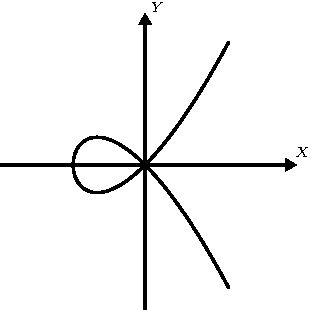
\includegraphics{diagram1-4.pdf}
    \end{center}
    What if we take the integral closure of $R$ in $\text{Frac}(R)$? It must contain $f=\frac{y}{x}$. Let $\ol{R}=R[f]$, which is a subring of $\text{Frac}(R)$. We claim that $\ol{R}$ is the integral closure of $R$ in $\text{Frac}(R)$. Notice that $\ol{R}\cong \CC[t]$ where $t$ is the image of $f$. So $\ol{R}$ is a UFD, so $\ol{R}$ is normal. So $\ol{R}$ is integrally closed in $\text{Frac}(\ol{R})=\text{Frac}(R)$. The affine space of $\ol{R}$ is $\AA^1$, which is the normalization of $X$. So we see that taking integral closure can somehow remove the singularity of the variety.
\end{example}
\begin{proposition}
    Let $R$ be an integral domain, $R\subseteq R'$ be a ring extension, $K$ be the field of fractions of $R$, and $S$ be a multiplicative closed subset of $R$.
    \begin{enumerate}
        \item If $\ol{R}$ is the integral closure of $R$ in $R'$, then $S\inv \ol{R}$ is the integral closure of $S\inv R$ in $S\inv R'$. In particular, if $R$ is normal, then $S\inv R$ is normal.
        \item If $R_{\km}$ is normal for all maximal ideals $\km$ of $R$, then $R$ is normal.
        \item If $R$ is normal, then $R[x]$ is normal. In fact, $R[x]$ is very closed to UFD, any monic irreducible polynomial in $R[x]$ is prime. 
    \end{enumerate}

\end{proposition}
\begin{proof}
    We give a proof for (3): if $R$ is normal, then $R[x]$ is normal. Let $K=\text{Frac}(R)$. Let $f/g$ be an element in $K(x)$ that is integral over $R[x]$, therefore integral over $K[x]$. Since $K[x]$ is normal, $f/g\in K[x]$. So we can write $p(x)=f/g=a_0+a_1x+\cdots + a_nx^n$ where $a_i\in K$. Since $h$ is integral over $R[x]$, $R[x,h]=R[a_0, a_1, \ldots, a_n,x]$ is integral over $R[x]$. So $R[x]/(x)\subseteq R[a_0, a_1, \ldots, a_n,x]/(x)=R[a_0, a_1, \ldots, a_n]$ is integral. Since $R[x]/(x)\cong R$ is normal, $a_0, a_1, \ldots, a_n\in R$, so $f/g\in R[x]$. Thus, $R[x]$ is normal.
\end{proof}
\begin{proposition}
   Let $R\subseteq R'$ be an extension of integral domains. If $R$ is integrally closed in $R'$, then for any monic $f,g\in R'[x]$ such that $fg\in R[x]$, we have $f, g\in R[x]$. 
   \\
   In particular, if $R$ is normal, then for any monic $f,g\in \text{Frac}(R)[x]$ such that $fg\in R[x]$, we have $f, g\in R[x]$ (Gauss Lemma). 
\end{proposition}
\begin{proof}
    Since $R$ is integral domain, $fg\in R[x]$ has finitely many roots in the algebraic closure of $K$ of $R'$. Since $fg$ is monic over $R$, we can adjoint all the roots $r_1, \ldots, r_n\in K$ of $fg$ to $R$ to get $S=R[r_1, \ldots, r_n]$. Notcie that any coefficient of $f$ and $g$ is the combination of $r_1, \ldots, r_n$ and is in $R'\subseteq K$, all the coefficients of $f$ and $g$ are integral over $R$. Since $R$ is integrally closed in $R'$, all the coefficients of $f$ and $g$ are in $R$, so $f, g\in R[x]$. 
\end{proof}
\begin{lemma}
    Let $R\subseteq R'$ be an integral extension of integral domains. If $R$ is normal, then 
    \begin{enumerate}
        \item For any $a\in R'$, its minimal polynomial over $K=\text{Frac}(R)$ has coefficients in $R$.
        \item If $a\in PR'$ for some prime ideal $P$ of $R$, then all the non-leading coefficients of the minimal polynomial of $a$ over $K$ are in $P$.
    \end{enumerate}
\end{lemma}
\begin{proof}[Proof of the lemma]
    \begin{enumerate}
        \item Let the monic minimal polynomial of $a$ over $K$ be $m$. And $a$ is integral over $R$, so there exists some monic polynomial $f\in R[x]$ such that $f(a)=0$. So $m$ divides $f$ in $K[x]$. Since both $m$ and $f$ are monic and $f/m\cdot m=f$, by the previous proposition, both $m$ and $f/m$ have coefficients in $R$. So $m$ has coefficients in $R$.
        \item Let $m(x)=x^n+a_{n-1}x^{n-1}+\cdots + a_0$ be the monic minimal polynomial of $a$ over $K$. If $a\in PR'$, then $\times a: R'\to R'$ is a map of $R$-modules such that $\times a(R')\subseteq PR'$. So we can apply the Cayley-Hamilton theorem to $\times a$ and $I=P$, we get some monic polynomial $f(x)=x^n+p_{n-1}x^{n-1}+\cdots + p_0\in R[x]$ such that $f(a)=0$ as an endomorphism of $R'$ and $p_i\in P$, so $f(a)1=0$ in $R'$, so $f(a)=0$ in $R'$. So there exists $h(x)\in R[x]$ such that $f(x)=h(x)m(x)$. Consider mod $P$, we have $\ol{x}^n=\ol{h}\ol{m}$ in $(R/P)[x]$. Since $R/P[x]$ is integral domain, $\ol{m}$ must be $\ol{x}^n$, so all the non-leading coefficients of $m$ are in $P$.
    \end{enumerate}
\end{proof}
\begin{remark}
    This lemma gives us a way to determine whether an element $a$ is integral over $R$ by looking at the coefficients of its minimal polynomial over $K$. 
\end{remark}

\begin{example}
    Consider $d$ a nonzero square-free integer. We can use this lemma to the integral closure of $\ZZ$ in $\QQ(\sqrt{d})$. We can show that the integral closure of $\ZZ$ in $\QQ(\sqrt{d})$ is $\ZZ[\frac{1+\sqrt{d}}{2}]$ if $d\equiv 1\mod 4$ and $\ZZ[\sqrt{d}]$ otherwise.
\end{example}
\subsection{Four Theorems}
For any morphism of affine varieties $f: X\to Y$, we have the corresponding morphism of coordinate rings $f^*: \CC[Y]\to \CC[X]$. It's easy to see that if $f$ is surjective, then $f^*$ is injective. Similarly, if $f^*$ is surjective, then $f$ is injective. However, when $f^*$ is injective, $f$ may not be surjective in general. For example, consider the inclusion from $k[x]$ to $k[x,y]/(xy)$, which corresponds to the morphism from $V(xy)$ to $\AA^1$ given by $(x,y)\mapsto x$. This morphism is not surjective since the image does not contain $0$, but the corresponding morphism of coordinate rings is injective. So we need some extra condition to guarantee that $f^*$ is injective implies $f$ is surjective. The extra condition turns out to be the integrality of $f^*$.
\\

\begin{theorem}[Lying Over]
    Let $R\subseteq R'$ be an integral extension of rings. Then for any prime ideal $P$ of $R$, there exists some prime ideal $P'$ of $R'$ such that $P'\cap R=P$.
\end{theorem}
\begin{proof}
    We will show a stronger result: 
    \begin{lemma}
        let $R\subseteq R'$ be an arbitary extension of rings and $P$ be a prime ideal of $R$. There exists $P'\subseteq R'$ such that $P'\cap R=P$ if and only if $PR'\cap R=P$. 
        \begin{subproof}[Subproof of the lemma]
            One direction is trivial. Conversely, if $PR'\cap R=P$, let $S=R\sm P$. So $S\cap PR'=\emptyset$. So we can localize at $S$ and $PR'$ becomes a proper ideal of $S\inv R'$. So there exists a maximal ideal $\km$ of $S\inv R'$ containing $S\inv PR'$. So there exists $P'$ of $R'$ such that $P'\cap S$ and $PR'\subseteq P'$. So $P=RP'\cap R\subseteq P'\cap R$. On the other hand, $P'\cap S=\emptyset$, so $P'\cap R\subseteq P$. So $P'\cap R=P$.
        \end{subproof}
        
    \end{lemma}
    When $R\subseteq R'$ is an integral extension, when for any prime $P\subseteq R$, $P\subseteq PR'\cap R$ is always true. For any $a\in PR'\cap R$, by Cayley-Hamilton theorem, there exists some monic polynomial $f(x)=x^n+p_{n-1}x^{n-1}+\cdots + p_0\in R[x]$ such that $f(a)=0$ and $p_i\in P$. Since $a\in R$, $a^n=-p_{n-1}a^{n-1}-\cdots - p_0\in P$, so $a\in P$. So $PR'\cap R=P$. Thus, we can apply the lemma to get some prime ideal $P'$ of $R'$ such that $P'\cap R=P$.
\end{proof}
\begin{remark}
    Given a integral extension from $i: \SO(Y)$ to $\SO(X)$, we have a morphism $\pi: X\to Y$. For any maximal ideal $\km$ of $\SO(Y)$, which corresponds to a point $Y'\in Y$, there exists some prime ideal $\kp'$ of $\SO(X)$ such that $\kp'\cap \SO(Y)=\km$. Geometrically, this is saying that there exists some closed subset $X'=V(\kp)$ of $X$ that maps to $y$. So $\pi$ is surjective.
\[\begin{tikzcd}
	{\mathcal{O}(X)} && {\mathcal{O}(Y)} && X && Y \\
	\\
	{\frac{\mathcal{O}(X)}{\kp'}=\mathcal{O}(X')} && {\frac{\mathcal{O}(Y)}{\km}=\mathcal{O}(Y')} && {X'} && {Y'}
	\arrow[two heads, from=1-1, to=3-1]
	\arrow["{i}"', from=1-3, to=1-1]
	\arrow[two heads, from=1-3, to=3-3]
	\arrow["\pi", from=1-5, to=1-7]
	\arrow[from=3-3, to=3-1]
	\arrow[hook, from=3-5, to=1-5]
	\arrow[from=3-5, to=3-7]
	\arrow[hook, from=3-7, to=1-7]
\end{tikzcd}\]
\end{remark}

\begin{example}
    Consider $R=k[x]$ and $R'=\frac{k[x,y]}{(x^2-y^2)}$. 
    \begin{center}
        
\includegraphics[scale=0.7]{diagram1-1.pdf}
    \end{center}
\end{example}
\begin{example}
    Consider $R=k[x]$ and $R'=\frac{k[x,y]}{(xy-1)}$.
    \begin{center}
        
\includegraphics[scale=0.7]{diagram1-2.pdf}
    \end{center}
    Notice that the preimage of point $Q$ is empty, that is, there is no prime ideal of $R'$ that contracts to the maximal ideal corresponding to $Q$. This is because $R\subseteq R'$ is not an integral extension.
\end{example}
\begin{theorem}[Incomparability]
    Let $R\subseteq R'$ be an integral extension of rings and $P$ be a prime ideal of $R$. If $P'\subseteq Q'$ are two prime ideals of $R'$ such that $P'\cap R=Q'\cap R=P$, then $P'=Q'$.
\end{theorem}
\begin{proof}
    Consider the integral extension $R/P\subseteq R'/P'$. Notice that $Q'/P'$ is a prime ideal of $R'/P'$ that contracts to the zero ideal of $R/P$. We want to show $Q'\P'=0$. Let $a+P'\in Q'/P'$. Since $R/P\subseteq R'/P'$ is an integral extension, there exists some monic polynomial $f(x)=x^n+p_{n-1}x^{n-1}+\cdots + p_0\in (R/P)[x]$ such that $f(a+P')=0$ in $R'/P'$. Since $R/P[x]$ is integral domain, we may assume $p_0\neq 0$. Notice that $p_0=-\ol{a}^n-p_{n-1}\ol{a}^{n-1}-\cdots - p_1\ol{a}\in Q'/P'$, so $p_0\in Q'/P'\cap R/P=0$, so $f(x)=x$. So $a+P=0$ in $R'/P'$, so $a\in P'$. Thus, $Q'/P'=0$, so $Q'=P'$.
\end{proof}
\begin{example}
    Consider $R=k[x]$ and $R'=\frac{k[x,y]}{(xy)}$. 
    \begin{center}
        
\includegraphics[scale=0.7]{diagram1-3.pdf}
    \end{center}
    Notice that the preimage of point $Q$ contains infinitely many points and the whole y-Axis. This is not allowed by the incomparability theorem. So $R\subseteq R'$ is not an integral extension.
\end{example}
\begin{corollary}
    Let $R\subseteq R'$ be an integral extension of rings. 
    \begin{enumerate}
        \item If $R$ and $R'$ are integral domains, then $R$ is a field if and only if $R'$ is a field.
        \item A prime ideal $P'$ of $R'$ is maximal if and only if $P'\cap R$ is maximal in $R$.
        \item If $R$ and $R'$ are integral domains, then the field of fractions of $R'$ is algebraic over the field of fractions of $R$. In this case, any nonzero ideal of $R'$ contracts to a nonzero ideal of $R$.
    \end{enumerate}
For (2), it's saying that only points can map to points under a morphism of varieties induced by an integral extension. 
\\
For (3), given the integral extension $R\subseteq R'$, we have the corresponding surjective morphism of varieties $\pi: \Spec(R')\surjto \Spec(R)$. Since $R$ and $R'$ are integral domains, $\Spec(R)$ and $\Spec(R')$ are irreducible. Nonzero ideal of $R'$ corresponds to a proper closed subset of $\Spec(R')$. So this is saying that any proper closed subset of $\Spec(R')$ maps to a proper closed subset of $\Spec(R)$ under $\pi$. This is true because $\Spec(R)$ and $\Spec(R')$ are irreducible and have the same kurll dimension. And any proper closed subset of an irreducible variety has smaller dimension, so it can't map to the whole $\Spec(R)$ by diemnsion argument. 
\end{corollary}
\begin{theorem}[Going Up]
    Let $R\subseteq R'$ be an integral extension of rings and $P\subseteq Q$ be two prime ideals of $R$. If $P'\subseteq R'$ is a prime ideal such that $P'\cap R=P$, then there exists some prime ideal $Q'\subseteq R'$ such that $P'\subseteq Q'$ and $Q'\cap R=Q$.
\end{theorem}
This is a direct consequence of the lying over. 
\begin{example}
    Consider $R=k[x]$ and $R'=\frac{k[x,y]}{(xy-1)\cap(x,y)}$. 
    \begin{center}
        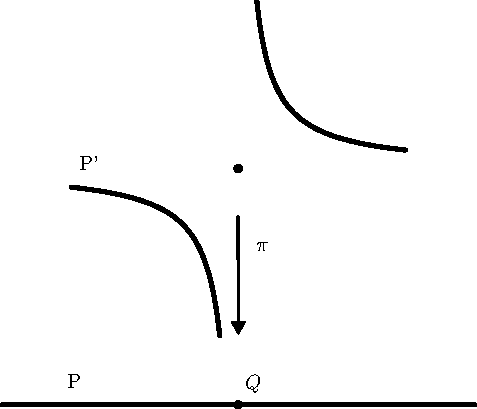
\includegraphics[scale=0.7]{diagram1-5.pdf}
    \end{center}
   Notice that this ring extension satisfys the incomparability and lying over theorems, but it does not satisfy the going up theorem: Given $P\subseteq Q$ in $R$ and $P'\subseteq R'$ such that $P'\cap R=P$, there is no prime ideal $Q'\subseteq R'$ such that $P'\subseteq Q'$ and $Q'\cap R=Q$, that is, there is no point in $P'$ that maps to point $Q$. We can more or less understand this geometrically: the fibers(preimages) of the morphism $\pi: \Spec(R')\to \Spec(R)$ should be sorta of continuous: a seqeunce of point in $R$ that converges to $Q$ should have preimages in $R'$ that converge to some point in the fiber of $Q$. 
\end{example}
\begin{theorem}[Going Down]
    Let $R\subseteq R'$ be an integral extension of rings and $R$ is normal domains and $R'$ is integral domains. If $P\subseteq Q$ are two prime ideals of $R$ and $Q'\subseteq R'$ is a prime ideal such that $Q'\cap R=Q$, then there exists some prime ideal $P'\subseteq R'$ such that $P'\subseteq Q'$ and $P'\cap R=P$.
\end{theorem}
\begin{remark}
    The going down theorem is not true if $R$ is not normal or if $R'$ is not integral domain. If $R'$ is not integral domain, say $R'=\frac{k[x,y]}{(x,y)\cap (y-1)}$, we can consider it as a line and a point not on the line. And $R=k[x]$. $R\subseteq R'$ is an integral extension. If we take $p=(0)$, $Q=(x)$ and $Q'=(x,y)$, then there is no prime ideal $P'\subseteq R'$ such that $P'\subseteq Q'$ and $P'\cap R=P$. This tells us $R'$ has to be irreducible/integral. 
    \begin{center}
        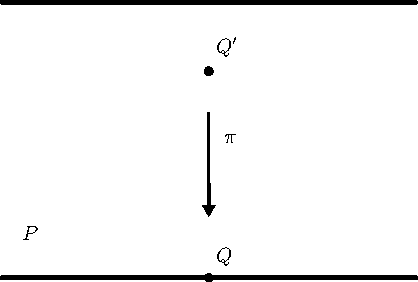
\includegraphics[scale=0.7]{diagram1-6.pdf}
    \end{center}
    The fact that $R$ has to be normal is a bit more subtle. We omit the counterexample here. 
\end{remark}
To summarize, the four theorems are saying that given an integral extension $R\subseteq R'$, we have a surjective morphism $\pi: \Spec(R')\surjto \Spec(R)$, and the fibers of $\pi$ well-behave in the sense that they are nonempty, finite, and sort of continuous. This implies the following theorem: 
\begin{theorem}
    If $R\to R'$ is an integral extension of rings, then $\dim(R)=\dim(R')$.
\end{theorem}
This is a direct consequence of the lying over and incomparability theorems.


\subsection{Some Special cases}
\begin{theorem}
    Let $R$ be a graded domain, then the integral closure of $R$ in its field of fractions is also a graded ring.
\end{theorem}
\begin{theorem}
    Let $\Gamma$ be a finitely generated semigroup in $\NN^n$ and $R=k[\Gamma]$ be the semigroup ring of $\Gamma$. Then the integral closure of $R$ in its field of fractions is $k[\overline{\Gamma}]$ where $\overline{\Gamma}=\RR_{\geq 0}\Gamma\cap \NN^n$. 
\end{theorem}
\subsection{Noether normalization and Nullstellensatz}
\begin{theorem}[Noether normalization]
    Let $R$ be a finitely generated algebra over a field $k$. Then there exists some algebraically independent elements $x_1, \ldots, x_d\in R$ such that $R$ is a finite extension of $k[x_1, \ldots, x_d]$. 
\end{theorem}
\begin{theorem}[Algberaic Nullstellensatz]
    Let $k$ be a field and $S$ be a finitely generated $k$-algebra. If $S$ is a field, then $S$ is a finite extension of $k$.
\end{theorem}
\begin{proof}
    By the Noether normalization, there exists some algebraically independent elements $x_1, \ldots, x_d\in S$ such that $S$ is a finite extension of $k[x_1, \ldots, x_d]$. Since $S$ is a field, $k[x_1, \ldots, x_d]$ is a field as well, so $d=0$. So $S$ is a finite extension of $k$. 
\end{proof}
\begin{theorem}[Weak Nullstellensatz]
    Let $k$ be an algebraically closed field and $\km$ be a maximal ideal of $k[x_1, \ldots, x_n]$. Then there exists some point $p=(a_1, \ldots, a_n)\in k^n$ such that $\km=(x_1-a_1, \ldots, x_n-a_n)$.
\end{theorem}
Consider $R=k[x_1, \ldots, x_n]/\km$ is a field and a finitely generated $k$-algebra, so by Noether normalization, there exists a polynomial ring $k[y_1, \ldots, y_d]$ such that $R$ is a finite extension of $k[y_1, \ldots, y_d]$. Since $R$ is a field, $k[y_1, \ldots, y_d]$ is a field as well, so $d=0$. So $R$ is a finite extension of $k$, so $R=k$. So $\km=(x_1-a_1, \ldots, x_n-a_n)$ for some $a_i\in k$.
\begin{theorem}[Strong Nullstellensatz]
    Let $k$ be an algebraically closed field and $I$ be an ideal of $k[x_1, \ldots, x_n]$. Then $\sqrt{I}=I(V(I))$.
\end{theorem}
\begin{proof}
\begin{lemma}
    For any ideal $I$ of $R=k[x_1, \ldots, x_n]$, \[\sqrt{I}=\bigcap_{\km\supseteq I}\km\] where $\km$ runs through all the maximal ideals of $k[x_1, \ldots, x_n]$ containing $I$.
    \begin{subproof}
        One direction is trivial. Conversely, if $f\notin \sqrt{I}$, we want to show that there exists some maximal ideal $\km$ of $k[x_1, \ldots, x_n]$ such that $I\subseteq \km$ and $f\notin \km$. So localize at $S=\{f^n: n\geq 0\}$, we get $S\inv I$ is a proper ideal of $S\inv k[x_1, \ldots, x_n]$. So there exists some maximal ideal $\km'$ of $S\inv k[x_1, \ldots, x_n]$ containing $S\inv I$. So there exists some prime ideal (not necessarily maximal) $\km$ of $k[x_1, \ldots, x_n]$ such that $\km\cap S=\emptyset$ and $\km\supseteq I$. We want to show that $\km$ is maximal. 
        \\

        Consider the extension $k\to R/\km \to R_f/\km_f$ (inclusion due to the fact that $R$ is integral domain). Notice that $R_f/\km_f$ is a field and it's a finitely generated $k$-algebra, so by the algebraic Nullstellensatz, $k\to R_f/\km_f$ is a finite extension. Therefore, $K\to R/\km$ is integral extension. So $R/\km$ is a field, so $\km$ is maximal.
    \end{subproof}
   
\end{lemma} Given the lemma, we can show that if $f\not\in \sqrt{I}$, then there exists some maximal ideal $\km$ of $k[x_1, \ldots, x_n]$ such that $I\subseteq \km$ and $f\notin \km$, so there exists some point $p\in V(I)$ such that $f(p)\neq 0$, so $f\notin I(V(I))$. The converse is trivial. 
\end{proof}
\begin{remark}
    The idea of the proof is that every algebraic set is a union of points, so we just need to show that every radical ideal is an intersection of maximal ideals.Therefore, we conclude the correspondence between algebraic sets and radical ideals.
\end{remark}
\newpage 
\section{March 12, 2026: Artin-Rees lemma and Krull's intersection theorem}
\subsection{Artin-Rees lemma}
\begin{definition}
    Given an ideal $I\subseteq R$. A sequence of $R$-modules $M=M_0\supseteq M_1\supseteq M_2\supseteq \cdots$ is called an $I$-filtration of $M$ if $IM_n\subseteq M_{n+1}$ for all $n\geq 0$.
    \\

    An $I$-filtration $M=M_0\supseteq M_1\supseteq M_2\supseteq \cdots$ is called $I$-stable if there exists some $n_0\geq 0$ such that $IM_n=M_{n+1}$ for all $n\geq n_0$.
\end{definition}
\begin{definition}
    A blowup algebra of $I$ in $R$ is the graded ring 
    \[B_IR=\bigoplus_{n\geq 0}I^n=R\oplus I\oplus I^2\oplus \cdots\cong R[tI]\subseteq R[t]\]
    \\

    Let $\mathcal{J} :M=M_0\supseteq M_1\supseteq M_2\supseteq \cdots$ be an $I$-filtration of $M$. We can define the blowup module of $\mathcal{J}$ as the graded $B_I(R)$-module: 
    \[B_{\mathcal{J}}M=\bigoplus_{n\geq 0}M_n=M\oplus M_1\oplus M_2\oplus \cdots\]
\end{definition}

    We may also define the associated graded ring with respect to $I$ as
    \[gr_IR=R/I\oplus I/I^2\oplus I^2/I^3\oplus \cdots\]
    We can easily see that $gr_IR\cong B_IR/IB_IR$. Similarly, we can define the associated graded module with respect to $\mathcal{J}$ as
    \[gr_{\mathcal{J}}M=M/M_1\oplus M_1/M_2\oplus M_2/M_3\oplus \cdots\]

\begin{proposition}
    This is our main proposition: Let $M$ be a finitely generated $R$-module and $\mathcal{J}: M=M_0\supseteq M_1\supseteq M_2\supseteq \cdots$ be an $I$-filtration of $M$. $B_{\mathcal{J}}M$ is a finitely generated $B_IR$-module if and only if $\mathcal{J}$ is $I$-stable.
\end{proposition}
\begin{proof}
    If $\mathcal{J}$ is $I$-stable, then we can easily generate $B_{\mathcal{J}}M$ by the generators of $M_0\oplus M_1\oplus \cdots \oplus M_{n_0}$. Conversely, if $B_{\mathcal{J}}M$ is a finitely generated $B_IR$-module, then we can find finitely many homogeneous elements that generate $B_{\mathcal{J}}M$ as a $B_IR$-module. So there must exists some $n$ such that all the generators are in $M_0\oplus M_1\oplus \cdots \oplus M_n$. Therefore, for any $M_{n+i}$ with $i\geq 0$, we can write any element in $M_{n+i}$ as a combination of the generators, so $M_{n+i}=I^iM_{n}$ for all $i>0$. So $\mathcal{J}$ is $I$-stable.
\end{proof}
\begin{theorem}[Artin-Rees lemma]
    Let $R$ be a Noetherian ring, $I$ be an ideal of $R$. If $M$ is a finitely generated $R$-module and $\mathcal{J}: M=M_0\supseteq M_1\supseteq M_2\supseteq \cdots$ is $I$-stable, then for any submodule $N\subseteq M$, the filtration $\mathcal{J}': N\cap M_0\supseteq N\cap M_1\supseteq N\cap M_2\supseteq \cdots$ is also $I$-stable. 
\end{theorem}
\begin{proof}
    Since $\mathcal{J}$ is $I$-stable, $B_{\mathcal{J}}M$ is a finitely generated $B_IR$-module. Since $R$ is Noetherian, $B_IR\subseteq R[t]$ is Noetherian. So $B_{\mathcal{J}}M$ is a Noetherian module, so any submodule of $B_{\mathcal{J}}M$ is finitely generated. In particular, $B_{\mathcal{J}'}N$ is a finitely generated $B_IR$-module, so $\mathcal{J}'$ is $I$-stable.
\end{proof}
\subsection{Krull's Intersection Theorem}
\begin{theorem}[Krull's intersection theorem]
    Let $I\subseteq R$ be an ideal of a Noetherian ring $R$ and $M$ be a finitely generated $R$-module. Then tehre exists $r\in I$ such that \[(1-r)(\bigcap_{n\geq 0}I^nM)=0\].
    In particular, if $R$ is local or integral domain, and $I$ is a proper ideal, then $\bigcap_{n\geq 0}I^nM=0$.
\end{theorem}
This is a direct consequence of the Artin-Rees lemma.
\begin{corollary}
    Let $R$ be a Noetherian ring and $I$ be a proper ideal of $R$. If $gr_IR$ is an integral domain, then $R$ is an integral domain as well.
\end{corollary}
For the proof, refer to Eisenbud's Commutative Algebra book, Corollary 5.5. 
\end{document}
